\documentclass[msc]{kou}

% Bazı temel bilgiler.
\makeatletter

% Kaynak dosyası.
\addbibresource{kaynaklar.bib}
% \addbibresource{kisisel.bib}   % kişisel yayın olunca açılacak
\addbibresource{kaynaklar-tez.bib}

% Başlık
\baslik{Bulut Platformlarında Log ve Metrik Korelasyonuna Dayalı Yapay Zekâ Destekli Proaktif Sağlık ve Kapasite Yönetimi}

% İngilizce başlık
\thetitle{AI-Assisted Proactive Health and Capacity Management Based on Log and Metric Correlation in Cloud Platforms}

% Yazar (Soyad Büyük yazılması gerekmektedir.)
\yazar{Yusuf KAYA}

% Anabilim dalı - departman
\bolum{Yazılım Mühendisliği}

% Tarih (TODO: teslim tarihine göre güncelle)
\tarihAY{}
\tarihYIL{2026}

% Savunma Tarihi (TODO: güncelle)
\starih{../../....}

% Jüri Üyeleri Adları ile Açıklamaları.
% (TODO: diğer jüri üyelerinin ünvan/adlarını doldur. Yüksek lisansta genellikle
%  3 üye bulunur; fazla satırları % ile kapatabilirsin.)
\jrBIR{Doç. Dr. Hakan GÜNDÜZ}
\jrBIRd{Danışman, Kocaeli Üniv.}

\jrIKI{Prof.Dr./Doç.Dr./Dr. Öğr. Üyesi}
\jrIKId{Jüri Üyesi, Kocaeli Üniv.}

\jrUC{Prof.Dr./Doç.Dr./Dr. Öğr. Üyesi}
\jrUCd{Jüri Üyesi, Kocaeli Üniv.}

\jrDORT{Prof.Dr./Doç.Dr./Dr. Öğr. Üyesi}
\jrDORTd{Jüri Üyesi, Kocaeli Üniv.}

\jrBES{Prof.Dr./Doç.Dr./Dr. Öğr. Üyesi}
\jrBESd{Jüri Üyesi, Kocaeli Üniv.}

\makeatother

% hyperref'in \autoref isimleri babel'ın ana dilini almaz ve İngilizce kalır
% ("Table 3.1", "Figure 3.1", "section 3.9"). TYK metin içi atıflarda "Tablo",
% "Şekil" ve "Bölüm" isimlerini zorunlu kıldığı için açıkça tanımlanır.
% Şekil arama yolu — cloudmon çıktıları make figures ile buraya kopyalanır
\graphicspath{{resimler/}}

\renewcommand{\figureautorefname}{Şekil}
\renewcommand{\tableautorefname}{Tablo}
\renewcommand{\chapterautorefname}{Bölüm}
\renewcommand{\sectionautorefname}{Bölüm}
\renewcommand{\subsectionautorefname}{Bölüm}

\begin{document}

\kapakolustur
\onayolustur

% Romen rakamlarının başlatılması
\clearpage
\pagenumbering{roman}

% Dizinleri  yazdırırken satır aralıklarının düzenlenmesi için
% grup içerisine alınmış ve düzenleme yapılmıştır. Ayrıca gerekli
% dizin isimlendirmeleri düzenlenmiştir.
\begingroup
\singlespacing

\etikolustur
\fikriolustur

\onsoz{Bu tez çalışması, Kubernetes ortamlarında ağ telemetrisi ve çalışma zamanı olaylarının birlikte analizine dayanan çok katmanlı bir anomali tespiti yaklaşımını konu almaktadır.

Çalışmanın planlanması ve yürütülmesi sürecinde bilgi ve desteğini esirgemeyen danışmanım Sayın Doç. Dr. Hakan Gündüz'e teşekkür ederim.

Bu süreçte maddi ve manevi desteklerini her zaman hissettiğim aileme teşekkür ederim.
}
\onsozolustur

\renewcommand{\listfigurename}{Şekiller Dizini}
\renewcommand{\listtablename}{Tablolar Dizini}
\tableofcontents
\listoffigures
\listoftables

\chapter*{Simgeler ve Kısaltmalar Dizini}
\tocless\section{Simgeler}
% TYK §2.1.9 + Ek-8: Simgeler alfabetik sıralanır ve **birimleri belirtilir**.
% Format: "simge : Açıklama, (birim)". Birimsiz (boyutsuz) niceliklerde birim
% yerine "(boyutsuz)" yazılır.
%
% Sıralama: Latin harfler (alfabetik), ardından Yunan harfleri.
\begin{simge}
	\item [$F_1$]          F1 skoru, (boyutsuz)
	\item [$h$]            Tahmin ufku, (saat)
	\item [$L$]            Kayıp fonksiyonu değeri, (boyutsuz)
	\item [$n$]            Gözlem sayısı, (adet)
	\item [$P$]            Kesinlik (precision), (boyutsuz)
	\item [$R$]            Duyarlılık (recall), (boyutsuz)
	\item [$R^2$]          Belirleme katsayısı, (boyutsuz)
	\item [$s$]            Log anomali skoru, (boyutsuz)
	\item [$T$]            Zaman penceresi uzunluğu, (saat)
	\item [$y$]            Gerçek kaynak kullanım değeri, (\%)
	\item [$\hat{y}$]      Tahmin edilen kaynak kullanım değeri, (\%)
	\item [$\theta$]       Kapasite alarm eşiği, (\%)
	\item [$\mu$]          Kayan ortalama, (boyutsuz)
	\item [$\phi$]         SHAP açıklama değeri, (boyutsuz)
	\item [$\sigma$]       Kayan standart sapma, (boyutsuz)
\end{simge}

\tocless\section{Kısaltmalar}
\addtocounter{section}{1}
% TYK §2.1.9 + Ek-8: alfabetik sıra; yabancı dildeki kısaltmaların Türkçe
% karşılığı **parantez içinde** verilir.
\begin{simge}
	\item [AI]     Artificial Intelligence (Yapay Zekâ)
	\item [AIOps]  Artificial Intelligence for IT Operations (BT Operasyonları için Yapay Zekâ)
	\item [API]    Application Programming Interface (Uygulama Programlama Arayüzü)
	\item [AUC]    Area Under the Curve (Eğri Altındaki Alan)
	\item [FN]     False Negative (Yanlış Negatif)
	\item [FP]     False Positive (Yanlış Pozitif)
	\item [GBT]    Gradient Boosted Trees (Gradyan Artırmalı Ağaçlar)
	\item [IaaS]   Infrastructure as a Service (Hizmet Olarak Altyapı)
	\item [IQR]    Interquartile Range (Çeyrekler Arası Aralık)
	\item [JSON]   JavaScript Object Notation
	\item [LGBM]   Light Gradient Boosting Machine (Hafif Gradyan Artırma Makinesi)
	\item [LLM]    Large Language Model (Büyük Dil Modeli)
	\item [LR]     Linear Regression (Doğrusal Regresyon)
	\item [MAE]    Mean Absolute Error (Ortalama Mutlak Hata)
	\item [MAPE]   Mean Absolute Percentage Error (Ortalama Mutlak Yüzdelik Hata)
	\item [ML]     Machine Learning (Makine Öğrenmesi)
	\item [MLP]    Multilayer Perceptron (Çok Katmanlı Algılayıcı)
	\item [RMSE]   Root Mean Squared Error (Kök Ortalama Kare Hata)
	\item [ROC]    Receiver Operating Characteristic (Alıcı İşletim Karakteristiği)
	\item [RF]     Random Forest (Rastgele Orman)
	\item [SHAP]   SHapley Additive exPlanations (Shapley Toplamsal Açıklamalar)
	\item [TSDB]   Time Series Database (Zaman Serisi Veritabanı)
	\item [TYK]    Tez Yazım Kılavuzu
	\item [VM]     Virtual Machine (Sanal Makine)
	\item [XAI]    Explainable Artificial Intelligence (Açıklanabilir Yapay Zekâ)
	\item [XGB]    eXtreme Gradient Boosting (Aşırı Gradyan Artırma)
\end{simge}


\ozet{Kubernetes tabanlı sistemlerde güvenlik gözlemlenebilirliği, mikroservisler arası yoğun ağ iletişimi ve kısa ömürlü çalışma yükleri nedeniyle geleneksel yöntemlerle sağlanamamaktadır. Bu tezde, ağ telemetrisi ve çalışma zamanı olaylarının birlikte analizine dayanan çok katmanlı bir anomali tespiti yaklaşımı araştırılmaktadır. Çalışma kapsamında, Kubernetes ortamında eBPF tabanlı Hubble aracı ile ağ akış verileri, Tetragon aracı ile çalışma zamanı olayları toplanmakta; bu veriler ön işleme ve özellik çıkarımı adımlarından geçirilerek katman bazlı gözetimsiz anomali tespit modelleri eğitilmektedir. Ağ ve çalışma zamanı katmanlarından elde edilen anomali skorları, her pod için birleşik bir güvenlik skoru üretmek üzere birleştirilmektedir. Yaklaşımın etkinliği, tek katmanlı modellerin hazır veri kümeleriyle doğrulanması ve çok katmanlı füzyonun kontrollü saldırı senaryolarıyla üretilen veriler üzerinde değerlendirilmesi yoluyla incelenecektir.}

\anahtarkelimeler{Anomali Tespiti, eBPF, Kubernetes, Makine Öğrenmesi, Siber Güvenlik.}
\ozetolustur

\theabstract{Security observability in Kubernetes-based systems cannot be achieved with traditional methods due to the intensive network communication among microservices and the short-lived nature of workloads. In this thesis, a multi-layer anomaly detection approach based on the joint analysis of network telemetry and runtime events is investigated. Within the scope of the study, network flow data are collected with the eBPF-based Hubble tool and runtime events with the Tetragon tool in a Kubernetes environment; these data are passed through preprocessing and feature extraction steps, and layer-specific unsupervised anomaly detection models are trained. The anomaly scores obtained from the network and runtime layers are combined to produce a unified security score for each pod. The effectiveness of the approach will be examined by validating the single-layer models on publicly available datasets and by evaluating the multi-layer fusion on data generated through controlled attack scenarios.}

\keywords{Anomaly Detection, eBPF, Kubernetes, Machine Learning, Cyber Security.}
\createabstract

\endgroup

% Latin/Arabic rakamların kullanılması
\clearpage
\pagenumbering{arabic}

% Bolumlerin eklenmesi
\chapter{GİRİŞ}
\label{ch:giris}

\section{Tezin Konusu ve Önemi}

Kurumsal ve akademik yapılarda giderek yaygınlaşan özel bulut altyapıları, büyük miktarda işlem, bellek ve depolama kaynağı barındırmaktadır.
Bu altyapıların sağlıklı biçimde işletilmesi; kaynak kullanımının takip edilmesini, arıza öncesi sinyallerin erkenden fark edilmesini ve operasyon ekiplerinin zamanında müdahale edebilmesini gerektirmektedir.
OpenStack \autocite{openstack2024}, açık kaynaklı mimarisi ve modüler bileşenleriyle (Nova, Neutron, Cinder, Keystone) özel bulut kurulumlarında tercih edilen önde gelen platformlardan biridir.

Geleneksel izleme yaklaşımları, metrik eşik değerlerini anlık olarak kontrol eden reaktif sistemlere dayanmaktadır.
Bu yaklaşım, yalnızca bir kaynak eşiği aştıktan sonra alarm üretmekte; operasyonel müdahale için yeterli zaman tanımamaktadır.
Oysa log verileri ve performans metrikleri birlikte değerlendirildiğinde, arıza veya kapasite aşımına ilişkin örüntüler genellikle saatler, hatta günler öncesinden gözlemlenebilmektedir.
Bu gerçeklik, log ve metrik korelasyonuna dayalı proaktif izleme yaklaşımlarını araştırmacılar ve uygulayıcılar için kritik bir alan haline getirmiştir \autocite{notaro2021}.

Yapay zekâ destekli BT operasyonları (AIOps) alanındaki çalışmalar, büyük ölçekli sistem log ve metriklerinden anlamlı örüntüler çıkarmak için makine öğrenmesi yöntemlerinin kullanılabileceğini göstermektedir \autocite{dang2019}.
Bununla birlikte, mevcut çalışmaların büyük çoğunluğu log analizi ya da metrik bazlı kapasite tahminini ayrı ayrı ele almakta; bu iki veri kaynağını tek bir karar destek çerçevesinde birleştiren uygulamalı çalışmalar ise sınırlı kalmaktadır.


\section{Problem Tanımı}

Özel bulut altyapılarında kaynak yönetimi birbirine bağlı birden fazla zorluk barındırmaktadır:

\begin{maddelendir}[label=\arabic*.]
    \item \textbf{Reaktif izleme sınırlaması:}
    Mevcut sistemler kaynak kullanımı eşiği aştığında alarm üretir; ancak o noktada operatörün müdahale süresi kısıtlanmıştır.
    Örneğin bellek kullanımı \%88 eşiğine yaklaştığında artık yeni sanal makine taleplerini karşılamak güçleşmektedir.

    \item \textbf{Log–metrik kopukluğu:}
    Log sistemleri (OpenSearch/Elasticsearch) ve metrik sistemleri (Prometheus/Thanos) ayrı araçlarla yönetilmekte, iki kaynak arasındaki ilişki çoğunlukla manuel incelemeye bırakılmaktadır.
    Bu kopukluk, \textit{slow\_response} ve \textit{memory\_pressure} gibi erken uyarı loglarının kapasite verileriyle ilişkilendirilmesini güçleştirmektedir.

    \item \textbf{Dönemsel yük artışları:}
    Staj dönemleri, sınav dönemleri ve eğitim kampanyaları gibi dönemsel olaylar kaynaklar üzerinde ani ve öngörülemeyen baskı yaratmaktadır.
    Bu baskılar, statik eşik tabanlı sistemler tarafından önceden saptanamamaktadır.

    \item \textbf{Açıklanabilirlik eksikliği:}
    Tahmin modelleri genellikle "kara kutu" olarak çalışmakta; hangi sinyalin kapasiteyi ne ölçüde etkilediği operatörlere aktarılamamaktadır.
    Bu durum model çıktılarına güveni zayıflatmaktadır.
\end{maddelendir}


\section{Tezin Amacı ve Kapsamı}

Bu tezin amacı, OpenStack tabanlı özel bulut altyapısı için log ve metrik korelasyonuna dayalı, yapay zekâ destekli proaktif bir sağlık ve kapasite yönetim sistemi (Bulut İzleme ve Öneri Sistemi) geliştirmek ve deneysel olarak değerlendirmektir.

Sistem, Ocak 2025 -- Temmuz 2026 (18 ay, 13.104 saatlik nokta) dönemine ait OpenStack metrik ve log verisi üzerinde altı adımlı bir pipeline çerçevesinde çalışmaktadır:

\begin{maddelendir}[label=\textbf{Adım \arabic*.}]
    \item \textbf{Veri Yükleme:} Prometheus/Thanos kaynaklı saatlik metrikler ile OpenSearch kaynaklı log özellik tablosu okunur.

    \item \textbf{Log İşleme Hattı:} Dört aşamalı log analizi yürütülür: (i) ayrıştırma ve tip sınıflandırması, (ii) zamansal agregasyon ve z-skor hesabı, (iii) anomali tespiti, (iv) ön-arıza örüntü çıkarımı.

    \item \textbf{Özellik Mühendisliği:} Metrik ve log sayımlarından 272 özellik üretilir (hareketli ortalama/std, gecikme, değişim hızı, zaman özellikleri, erken uyarı bileşik sinyali).

    \item \textbf{Kapasite Tahmini:} Yedi farklı regresyon algoritması (LR, RF, GBT, XGB, LGBM, CatBoost, MLP) üç kaynak (vCPU, Bellek, Disk) için iki tahmin ufkunda (24 saat, 72 saat) eğitilerek toplam 42 model değerlendirilir.

    \item \textbf{SHAP Analizi:} Her model için özellik önem sıralaması TreeExplainer/LinearExplainer yöntemiyle hesaplanır; hangi metrik ya da log tipinin tahmine en çok katkıda bulunduğu yorumlanır.

    \item \textbf{Proaktif Öneri Üretimi:} Kural tabanlı öneri motoru ve iki büyük dil modeli (Claude Sonnet, GPT-4o) birleştirilerek operasyon ekibine önceliklendirilmiş, aksiyona dönüştürülebilir öneriler üretilir.
\end{maddelendir}

Çalışma kapsamı dışında bırakılanlar: gerçek zamanlı akış işleme (streaming), OpenStack altyapısının kurulumu ve yapılandırması, veri üretim süreçlerinin iyileştirilmesi.


\section{Tezin Katkıları}

Bu çalışmanın başlıca özgün katkıları şunlardır:

\begin{maddelendir}[label=\arabic*.]
    \item \textbf{Log--metrik korelasyonuna dayalı kapasite tahmini:}
    Literatürdeki çalışmaların büyük bölümü metrik ya da log verisini ayrı ele alırken, bu çalışmada her ikisi ortak bir özellik uzayında birleştirilerek kapasite tahminine katkısı ölçülmüştür.
    SHAP analizleri, \textit{resource\_exhausted} ve \textit{scheduler\_degradation} gibi log sayılarının kapasite tahmininde metrik özellikleriyle rekabet edebilir düzeyde etkili olduğunu ortaya koymaktadır.

    \item \textbf{Dört aşamalı log işleme pipeline'ı:}
    Ham log sayımlarından ön-arıza örüntülerine uzanan sistematik bir analiz hattı tasarlanmıştır.
    Bu hat, \textit{slow\_response} loglarının arızadan ortalama 68 saat önce anormal artış gösterdiği gibi içgörüler üretmektedir.

    \item \textbf{Açıklanabilir kapasite tahmin sistemi:}
    SHAP değerleri her tahmin için hesaplanmakta ve en etkili özellikler operatöre aktarılmaktadır.
    Bu yaklaşım, kara kutu model çıktılarını yorumlanabilir aksiyonlara dönüştürmektedir \autocite{lundberg2017, lundberg2020}.

    \item \textbf{Zenginleştirilmiş bağlamla LLM destekli öneri motoru:}
    Metrik durumu, log anomali sinyalleri, SHAP özellik önem sıralaması ve cascade riski birleştirilerek oluşturulan yapılandırılmış bağlam, Claude Sonnet ve GPT-4o modellerine iletilmektedir.
    Sistem, servis bazında önceliklendirilmiş ve uygulanabilir aksiyonlar üretmektedir \autocite{brown2020, openai2023}.
\end{maddelendir}


\section{Tez Organizasyonu}

Tez altı ana bölümden oluşmaktadır.
Birinci bölümde (Giriş) çalışmanın konusu, problemi, amacı ve katkıları özetlenmiştir.
İkinci bölümde (Genel Bilgiler) AIOps, bulut kapasite yönetimi, log analizi, açıklanabilir yapay zekâ ve büyük dil modelleri konularındaki ilgili literatür incelenmektedir.
Üçüncü bölümde (Malzeme ve Yöntem) Bulut İzleme ve Öneri Sisteminin mimarisi, kullanılan veri kümesi, özellik mühendisliği, model eğitimi ve öneri motoru ayrıntılandırılmaktadır.
Dördüncü bölümde (Bulgular) 42 modelin karşılaştırmalı sonuçları, SHAP analizleri ve öneri motoru çıktıları sunulmaktadır.
Beşinci bölümde (Sonuçlar ve Öneriler) elde edilen bulgular değerlendirilmekte, çalışmanın sınırlılıkları tartışılmakta ve gelecek çalışma önerileri sunulmaktadır.

\chapter{GENEL BİLGİLER}
\label{ch:genelbilgiler}

Bu bölümde tez çalışmasının kavramsal altyapısını oluşturan konular ele alınmaktadır.
Önce yapay zekâ destekli BT operasyonları (AIOps) kavramı ve bulut platformlarındaki kapasite yönetimi sorunları sunulmaktadır.
Ardından log analizi ve anomali tespiti yöntemleri incelenmekte, makine öğrenmesi modelleri ile açıklanabilir yapay zekâ yaklaşımları tartışılmaktadır.
Son olarak büyük dil modellerinin operasyonel zekayla entegrasyonu ve literatürdeki açık noktalar değerlendirilerek tezin konumlandığı alan belirlenmektedir.


\section{Yapay Zekâ Destekli BT Operasyonları (AIOps)}

BT sistemlerinin ölçeği büyüdükçe operasyonel verilerin hacmi (log, metrik, olay akışları) insan kapasitesinin çok üzerine çıkmaktadır.
Bu gerçeklik, makine öğrenmesi ve büyük veri tekniklerini BT operasyonları süreçlerine entegre eden AIOps (Artificial Intelligence for IT Operations) yaklaşımını doğurmuştur \autocite{dang2019}.

Notaro ve arkadaşları, AIOps literatürünü kapsamlı biçimde inceleyerek başarısızlık yönetimi için kullanılan yöntemleri anomali tespiti, kök neden analizi ve olay korelasyonu başlıkları altında sınıflandırmıştır \autocite{notaro2021}.
Bu sınıflandırmaya göre proaktif kapasite yönetimi, anomali tespitinin özel bir formu olarak değerlendirilebilir: kaynak kullanımının belirli bir eşiği aşmadan önce örüntüden sapması tespit edilerek önleyici aksiyon alınır.

AIOps'un başarısı büyük ölçüde veri kalitesine ve farklı kaynaklardan gelen sinyallerin etkin biçimde birleştirilmesine bağlıdır.
Metrikler, kesintisiz sayısal sinyal sağlarken; loglar, hata türleri, uyarı desenleri ve servis sağlık durumu hakkında metriklerin içermediği bağlamsal bilgi sunar.
Bu iki kaynağın korelasyonu, tek kaynaklı yaklaşımlara kıyasla daha erken ve daha kesin uyarı üretilmesine olanak tanımaktadır.


\section{Bulut Altyapılarında Kapasite Yönetimi}

Kapasite yönetimi, mevcut altyapının talepleri karşılamaya devam edip etmeyeceğini öngörme ve buna göre planlama yapma sürecidir.
Bulut ortamlarında bu süreç; vCPU, bellek ve disk gibi temel kaynakların kullanım trendlerinin izlenmesini ve gelecekteki tüketimin tahmin edilmesini kapsamaktadır.

Geleneksel yaklaşımlar iş yükü tahmininde ARIMA ve üstel düzeltme gibi istatistiksel zaman serisi yöntemlerine dayanmaktadır \autocite{calheiros2015}.
Bu yöntemler durağan ve periyodik örüntülü verilerde başarılı olurken, staj dönemleri ve anlık yük artışları gibi düzensiz olayları içeren bulut iş yüklerinde yetersiz kalabilmektedir.

Makine öğrenmesi yöntemleri bu sınırlılığı aşmak için önerilmiştir.
Özellik mühendisliği yoluyla geçmiş pencere istatistikleri, gecikme değerleri ve takvim bilgileri (iş günü, saat) modele dahil edilerek zaman serisi tahmini bir regresyon problemine dönüştürülmektedir.
Bu yaklaşımda her gözlem noktası, geçmiş zaman penceresinden türetilen özellik vektörüyle temsil edilmekte ve model bu vektörden gelecekteki kaynak kullanımını tahmin etmektedir.

OpenStack tabanlı özel bulut altyapılarında Nova (işlem), Cinder (depolama), Neutron (ağ) ve Keystone (kimlik) bileşenleri, Prometheus/Thanos ile saatlik metrik akışı sağlayarak makine öğrenmesi destekli kapasite yönetiminin veri altyapısını oluşturmaktadır \autocite{openstack2024}.


\section{Log Analizi ve Anomali Tespiti}

Log verileri, sistem olaylarının zaman damgalı metin kaydıdır.
Ham loglardan kapasite yönetimine anlamlı girdi oluşturmak birkaç aşamalı bir işlemi gerektirir: ayrıştırma ve sınıflandırma, zamansal agregasyon, anomali tespiti ve ön-arıza örüntü çıkarımı.

He ve arkadaşları, log ayrıştırma algoritmalarını kapsamlı biçimde değerlendirerek Drain, Spell ve AEL gibi yöntemlerin gerçek dünya log verisi üzerindeki etkinliğini karşılaştırmıştır \autocite{he2016}.
Log analizi için otomasyon yaklaşımlarını inceleyen daha kapsamlı bir tarama çalışması, ayrıştırma, kümeleme, sınıflandırma ve anomali tespiti adımlarını birleştiren bütünleşik pipeline yaklaşımlarının etkinliğini ortaya koymaktadır \autocite{he2021}.

Anomali tespiti açısından Chandola ve arkadaşları, noktasal, bağlamsal ve kolektif anomaliler arasındaki ayrımı tanımlayarak istatistiksel, kümeleme tabanlı ve sınıflandırma tabanlı yöntemleri sistematik biçimde sınıflandırmıştır \autocite{chandola2009}.
Derin öğrenme tabanlı yaklaşımlar ise özellikle yüksek boyutlu ve yapılandırılmamış veriler için güçlü alternatifler sunmaktadır \autocite{pang2021}.

Log dizisi anomali tespitinde önemli bir dönüm noktası olan DeepLog, sistem loglarını LSTM modeli ile modelleyerek normal log dizilerinden sapmaları tespit etmekte ve tanılamaktadır \autocite{du2017}.
Log verisi için derin öğrenme yaklaşımlarını derleyen güncel bir tarama çalışması, denetimsiz ve yarı denetimli yöntemlerin üretim ortamlarındaki kararsız log formatlarına karşı daha dayanıklı olduğunu göstermektedir \autocite{landauer2023}.

Bulut platformlarında loglar yalnızca hata bildirmez; arızadan saatler önce ortaya çıkan \textit{yavaş yanıt}, \textit{bellek baskısı} ve \textit{bağlantı havuzu uyarısı} gibi erken uyarı sinyalleri de içerir.
Bu sinyallerin zamansal örüntülerinin çıkarılması ve metrik verisiyle korelasyonu, proaktif izlemenin temel katkısını oluşturmaktadır.


\section{Makine Öğrenmesi ile Zaman Serisi Regresyonu}

Kapasite tahmini bu çalışmada bir regresyon problemi olarak ele alınmaktadır: geçmiş özellik vektörü verildiğinde $h$ saat sonraki kaynak kullanım oranı $\hat{y}$ tahmin edilmektedir.

\textbf{Doğrusal Regresyon (LR):}
Özellik vektörünün doğrusal kombinasyonuyla hedef değişkeni modelleyen temel yöntemdir.
Yorumlanabilirliği yüksektir; ancak doğrusal olmayan ilişkileri yakalayamaz.
Bu çalışmada StandardScaler ile normalizasyon uygulanmaktadır.

\textbf{Rastgele Orman (RF):}
Breiman tarafından önerilen topluluk öğrenmesi yöntemidir \autocite{breiman2001}.
Birbirinden bağımsız karar ağaçlarının tahminlerini ortalaması alarak oluşturur; aşırı öğrenmeye karşı dayanıklıdır ve özellik önem skoru hesaplamaya doğrudan olanak tanır.

\textbf{Gradyan Artırmalı Ağaçlar (GBT):}
Friedman tarafından geliştirilen ve artık (residual) tabanlı sıralı ağaç inşa eden yöntemdir \autocite{friedman2001}.
XGBoost \autocite{chen2016}, LightGBM \autocite{ke2017} ve CatBoost \autocite{prokhorenkova2018} bu temel yöntemin hesaplama verimliliğini ve doğruluğunu artıran modern uygulamalarıdır.

\textbf{Çok Katmanlı Algılayıcı (MLP):}
İleri beslemeli yapay sinir ağıdır.
Doğrusal olmayan ilişkileri yakalama kapasitesi yüksektir; ancak hiperparametre ayarı ve eğitim süresi diğer yöntemlere kıyasla daha fazla dikkat gerektirir.
Bu çalışmada StandardScaler ile normalizasyon uygulanmaktadır.

Model performansı dört metrikle değerlendirilmektedir: MAE (Ortalama Mutlak Hata), RMSE (Kök Ortalama Kare Hata), R\textsuperscript{2} (Belirleme Katsayısı) ve MAPE (Ortalama Mutlak Yüzdelik Hata).
Bu metrikler hem mutlak hata büyüklüğünü (MAE, RMSE) hem de varyansın ne kadarının model tarafından açıklandığını (R\textsuperscript{2}) ve yüzdesel sapmayı (MAPE) birlikte değerlendirmeye olanak tanımaktadır.


\section{Açıklanabilir Yapay Zekâ ve SHAP}

Makine öğrenmesi modellerinin karar destek süreçlerinde kullanılabilmesi için operatörlerin model çıktılarını anlayabilmesi kritik önem taşımaktadır.
Açıklanabilir yapay zekâ (XAI), kara kutu modellerin tahminlerini yorumlanabilir kılmayı hedeflemektedir.

SHAP (SHapley Additive exPlanations), oyun teorisindeki Shapley değerlerinden türetilen tutarlı bir özellik atıf yöntemidir \autocite{lundberg2017}.
Her özelliğin modelin tahmine katkısı, o özelliğin dahil edilip edilmediği tüm alt kümelerin kombinasyonları üzerinden hesaplanmakta; bu sayede hem yerel (tek tahmin) hem de global (tüm veri seti) açıklamalar üretilebilmektedir.

Ağaç tabanlı modeller için önerilen TreeSHAP algoritması, polinom zamanlı naif SHAP hesabını üstel karmaşıklıktan polinom karmaşıklığa indirerek büyük ölçekli modellerde uygulanabilir kılmaktadır \autocite{lundberg2020}.
Doğrusal modeller için ise LinearExplainer, katsayıların beklenti değerinden sapmasını doğrudan hesaplar; model-agnostik Kernel SHAP ise MLP gibi kara kutu modellerle kullanılır.

Bu çalışmada SHAP analizi üç amaçla kullanılmaktadır:
(i) hangi metrik ve log özelliklerinin kapasite tahminini en çok etkilediğinin belirlenmesi,
(ii) log sayımlarının metrik özelliklerle rekabet eden tahmin katkısının ölçülmesi ve
(iii) operatörlere üretilen önerilerin dayandığı kanıtların aktarılması.


\section{Büyük Dil Modelleri ve Operasyonel Zekâ}

Büyük dil modelleri (LLM), milyarlarca parametreli dönüştürücü (transformer) mimarisiyle eğitilen ve doğal dil anlama ile üretme kapasitesine sahip modellerdir.
GPT-3 \autocite{brown2020} ile birlikte bağlam içi öğrenme (in-context learning) kapasitesi gösterilmiş; GPT-4 \autocite{openai2023} ve Claude \autocite{anthropic2024} ile bu kapasite üretim ortamlarında kullanılabilir düzeye ulaşmıştır.

IT operasyonları alanında LLM'ler, yapılandırılmış sistem verilerini (metrik, log, uyarı) doğal dil önerilerine dönüştürme rolüyle kullanılmaktadır.
Bu yaklaşımın başarısı büyük ölçüde modele sağlanan bağlamın kalitesine bağlıdır: yalnızca ham metrik değerlerinin iletilmesi yerine, SHAP özellik önem sıralaması, log anomali sinyalleri, tahmin ufku ve servis sağlık durumu gibi bağlamsal bilgilerin eklenmesi daha spesifik ve uygulanabilir öneriler üretilmesini sağlamaktadır.

Bu çalışmada Claude Sonnet ve GPT-4o modelleri paralel olarak kullanılmakta; her iki modelin yanıtı tek bir operasyonel raporda birleştirilmektedir.
Modellere iletilen istem (prompt), kapasite durumu, log özeti, SHAP sıralaması, ön-arıza örüntüleri ve cascade risk skoru içeren yapılandırılmış bir bağlam bloğunu kapsamaktadır.


\section{Literatürdeki Boşluk ve Tezin Konumlandığı Alan}

İncelenen çalışmalar değerlendirildiğinde şu eksiklikler göze çarpmaktadır:

\begin{maddelendir}[label=\arabic*.]
    \item Mevcut AIOps çalışmalarının büyük bölümü log analizi ya da metrik bazlı kapasite tahminini ayrı ayrı ele almaktadır.
    Her iki veri kaynağını tek bir özellik uzayında birleştiren ve korelasyonun tahmini nasıl iyileştirdiğini nicel olarak ölçen uygulamalı çalışmalar sınırlı kalmaktadır.

    \item Ön-arıza örüntü çıkarımı (pre-failure pattern mining) kapasite tahminiyle birlikte ele alınmamaktadır.
    Geçmiş incident'lerin öncesindeki log imzalarının sistematik biçimde çıkarılıp gelecekteki uyarı üretimine katkı sağlaması literatürde yeterince araştırılmamıştır.

    \item SHAP analizinin kapasite yönetimi bağlamında uygulanması ve log özelliklerinin tahmin katkısının metrik özellikleriyle karşılaştırılması spesifik olarak ele alınmamıştır.

    \item LLM entegrasyonu genellikle log-to-text veya alert-to-text dönüşümlerine odaklanmaktadır.
    Metrik, log, SHAP ve cascade bilgisini birleştiren zenginleştirilmiş bağlam ile proaktif öneri üretimi yeterince araştırılmamıştır.
\end{maddelendir}

Bu tez, söz konusu boşlukları hedef alarak OpenStack tabanlı gerçek bir bulut altyapısı üzerinde log--metrik korelasyonuna dayalı, açıklanabilir ve LLM destekli proaktif bir kapasite yönetim sistemi geliştirmektedir.

\chapter{MALZEME VE YÖNTEM}
\label{ch:malzemeveyontem}

Bu bölümde CloudMon sisteminin geliştirildiği OpenStack deney ortamı, veri toplama altyapısı, sistem mimarisi, log işleme pipeline'ı, özellik mühendisliği, kapasite tahmin modelleri, SHAP analizi ve öneri motoru ayrıntılı olarak açıklanmaktadır.


\section{Sistem Mimarisi}

CloudMon, OpenStack tabanlı özel bulut altyapısının proaktif olarak izlenmesi amacıyla geliştirilmiş altı adımlı bir analiz pipeline'ıdır.
Sistemin genel mimarisi \autoref{fig:mimari}'de gösterilmektedir.

\begin{figure}[htbp]
    \centering
    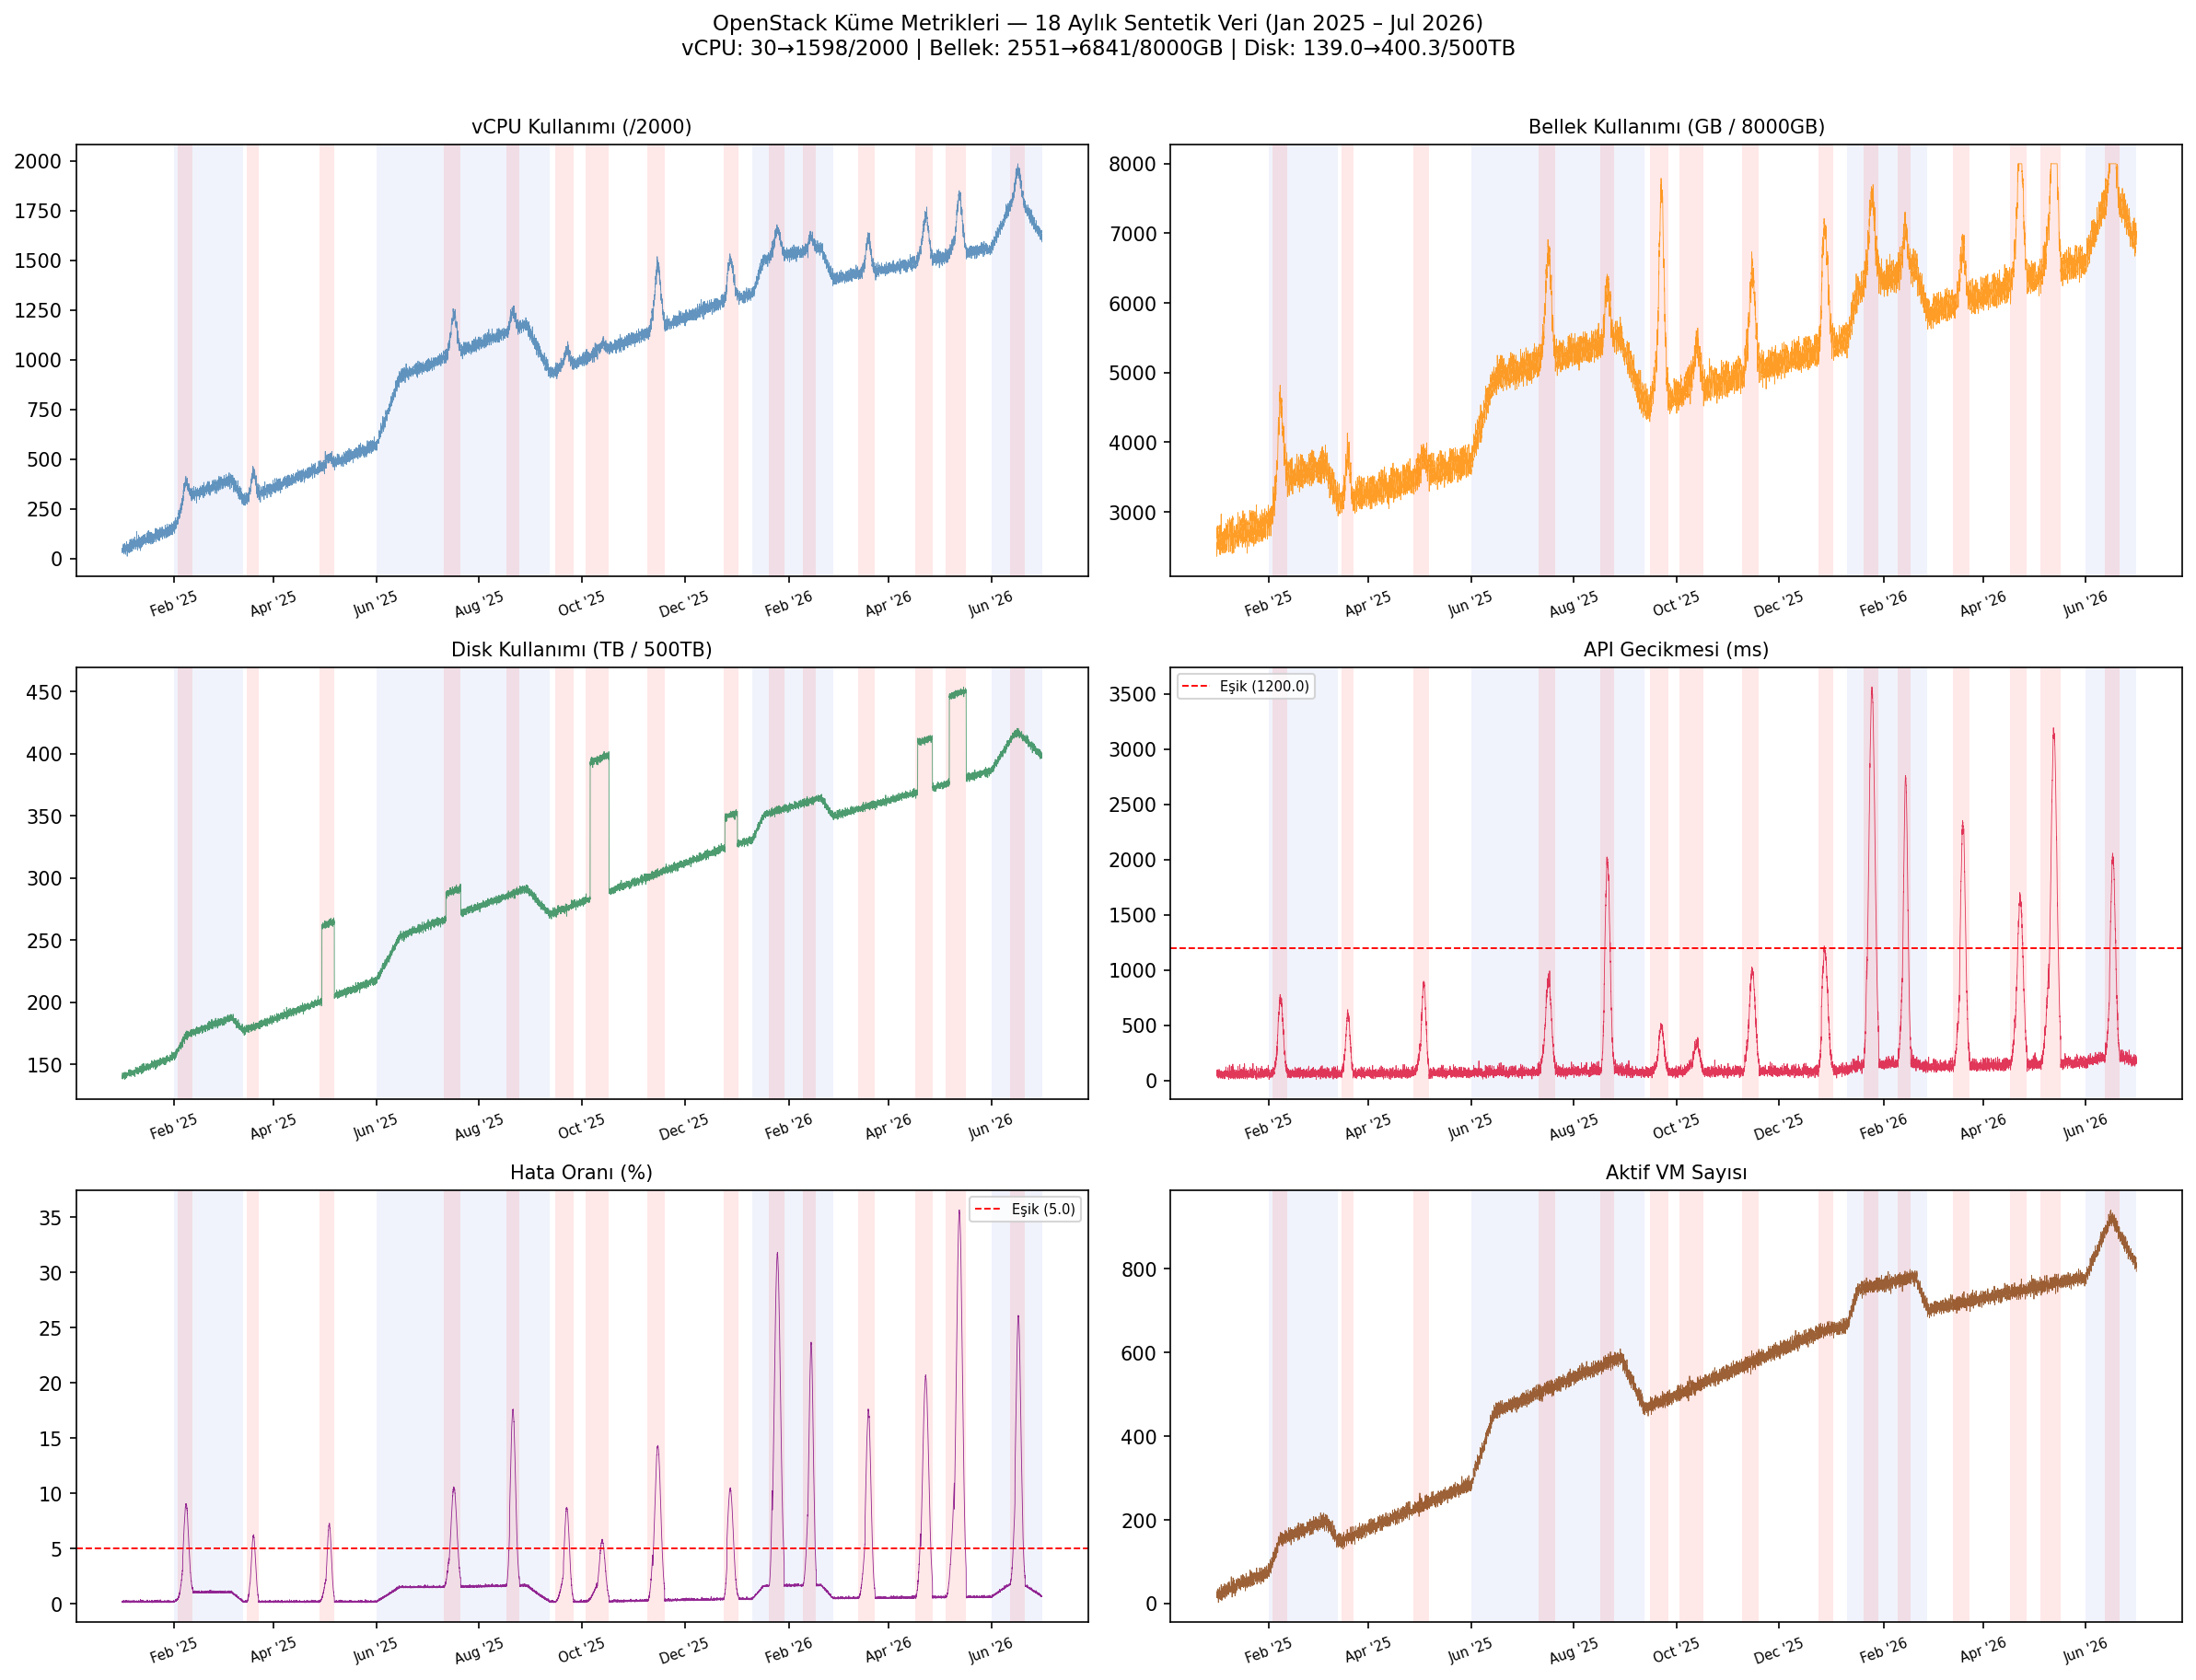
\includegraphics[width=0.95\textwidth]{metrics_overview}
    \caption{CloudMon pipeline'ının genel akışı: veri yükleme, log analizi, özellik mühendisliği, kapasite tahmini, SHAP analizi ve öneri üretimi.}
    \label{fig:mimari}
\end{figure}

Pipeline adımları sırasıyla şunlardır:
\begin{maddelendir}[label=\textbf{Adım \arabic*.}]
    \item \textbf{Veri Yükleme:} Prometheus/Thanos kaynaklı saatlik metrikler (\texttt{metrics.csv}) ve OpenSearch kaynaklı saatlik log özellik tablosu (\texttt{log\_features.csv}) okunur.
    \item \textbf{Log İşleme Hattı:} Dört aşamalı analiz gerçekleştirilir (bkz. \autoref{sec:logpipeline}).
    \item \textbf{Özellik Mühendisliği:} Metrik ve log verilerinden 272 özellik türetilir (bkz. \autoref{sec:ozellik}).
    \item \textbf{Kapasite Tahmini:} Yedi algoritma $\times$ üç kaynak $\times$ iki ufuk = 42 regresyon modeli eğitilir (bkz. \autoref{sec:modeller}).
    \item \textbf{SHAP Analizi:} Her model için özellik atıf değerleri hesaplanır (bkz. \autoref{sec:shap}).
    \item \textbf{Öneri Üretimi:} Kural tabanlı motor ve LLM çıktıları birleştirilerek operasyonel rapor oluşturulur (bkz. \autoref{sec:oneri}).
\end{maddelendir}


\section{Deney Ortamı ve Veri Toplama Altyapısı}
\label{sec:ortam}

\subsection{OpenStack Altyapısı}

CloudMon, TÜBİTAK BİLGEM bünyesinde geliştirilen OpenStack tabanlı özel bulut platformu üzerinde çalıştırılmıştır.
OpenStack, açık kaynak kodlu, modüler bir bulut işletim sistemi olup işlem, depolama ve ağ kaynaklarını API aracılığıyla yazılım katmanından yönetmeye olanak tanımaktadır \autocite{openstack2024}.
Bu çalışmada dört temel OpenStack servisi izleme kapsamına alınmıştır:

\begin{maddelendir}[label=--]
    \item \textbf{Nova (Compute):} Sanal makine yaşam döngüsünü yöneten işlem servisi.
    Kapasite açısından en kritik bileşendir: vCPU ve bellek kaynaklarının tahsisi, VM başlatma/durdurma işlemleri ve zamanlayıcı (scheduler) kararları bu servis tarafından gerçekleştirilmektedir.
    Nova, \texttt{nova-api}, \texttt{nova-compute} ve \texttt{nova-scheduler} alt servislerinden oluşmaktadır; bu alt servisler bağımsız olarak izlenmekte ve servis sağlık skorlarına ayrı ayrı katkı sağlamaktadır.

    \item \textbf{Neutron (Network):} Sanal ağları, alt ağları, yönlendiriciyi ve güvenlik gruplarını yöneten ağ servisidir.
    VM'ler arası ve dış ağ iletişimini sağlar; bant genişliği ve ağ hatası metrikleri bu servis üzerinden izlenmektedir.

    \item \textbf{Cinder (Block Storage):} Sanal makinelere bağlanan kalıcı blok depolama birimlerini yöneten depolama servisidir.
    Disk I/O hatası ve depolama kullanım oranı metrikleri Cinder bileşeninden elde edilmektedir.

    \item \textbf{Keystone (Identity):} Kullanıcı kimlik doğrulama, proje kota yönetimi ve servisler arası yetkilendirmeyi sağlayan kimlik servisidir.
    Kimlik doğrulama hataları ve kota aşımı uyarıları Keystone loglarından türetilmektedir.
\end{maddelendir}

\subsection{Metrik Toplama: Prometheus ve Thanos}

OpenStack servislerinden metrik verisi, Prometheus/Thanos izleme yığını aracılığıyla saatlik aralıklarla toplanmaktadır.
Prometheus, her servisten HTTP endpoint'ler üzerinden metrik kazıma (scraping) yaparak zamanlı metrik dizileri oluşturmaktadır.
Thanos bu yapının üzerine uzun vadeli depolama ve çok bölgeli (multi-region) sorgulama katmanı eklemektedir; bu sayede 18 aylık veri tutarlı biçimde sorgulanabilmektedir.

CloudMon, Prometheus/Thanos'tan saatlik granülarite ile \texttt{metrics.csv} formatında dokuz birincil metriği okumaktadır (\autoref{tab:metrikler}).
Metrik toplama süreci üç aşamadan oluşmaktadır: (i) Prometheus endpoint'lerinden ham verilerin kazınması, (ii) Thanos sorgu katmanı üzerinden saatlik agregasyonun gerçekleştirilmesi ve (iii) CSV formatına dönüştürülerek CloudMon veri dizinine yazılması.

\subsection{Log Toplama: OpenSearch}

OpenStack servis logları OpenSearch platformunda merkezi olarak depolanmaktadır.
Fluentd log iletim aracı, Nova, Neutron, Cinder ve Keystone servislerinin \texttt{/var/log/} çıktılarını gerçek zamanlı olarak OpenSearch endekslerine aktarmaktadır.

CloudMon log işleme için ham log satırlarını değil, önceden belirlenmiş 15 log tipi üzerinden saatlik pencere bazında hesaplanan sayımları kullanmaktadır (\texttt{log\_features.csv}).
Bu yaklaşım iki avantaj sağlamaktadır: birincisi, log hacmine bağlı hesaplama maliyetini sabit ve öngörülebilir kılmak; ikincisi, log ayrıştırma (parsing) adımını CloudMon dışında OpenSearch sorgu katmanında gerçekleştirerek pipeline'a temiz ve yapılandırılmış girdi sağlamak.

Saatlik log özellik tablosu şu şekilde üretilmektedir: her saat dilimi için her log tipi, ilgili OpenSearch endeksinde anahtar kelime eşleşmesiyle sorgulanmakta ve bulunan kayıt sayısı tek bir satıra yazılmaktadır.
Bu işlem \texttt{raw\_logs.csv} içindeki ham log örneklemesiyle desteklenmekte; ön-arıza örüntü çıkarımı (Aşama 4) ham loglar üzerinden çalıştırılmaktadır.

\subsection{Veri Akışı}

\autoref{fig:veriakisi}'de CloudMon'un uçtan uca veri akışı görülmektedir.
OpenStack servisleri → Prometheus/Thanos → \texttt{metrics.csv} hattı metrik verisi sağlarken, OpenStack servisleri → Fluentd → OpenSearch → \texttt{log\_features.csv} hattı log özellik tablosunu üretmektedir.
Her iki kaynak saatlik granülaritede CloudMon ana pipeline'ına beslenmekte; özellik mühendisliği adımında tek bir 272 boyutlu vektöre birleştirilmektedir.

\begin{figure}[htbp]
    \centering
    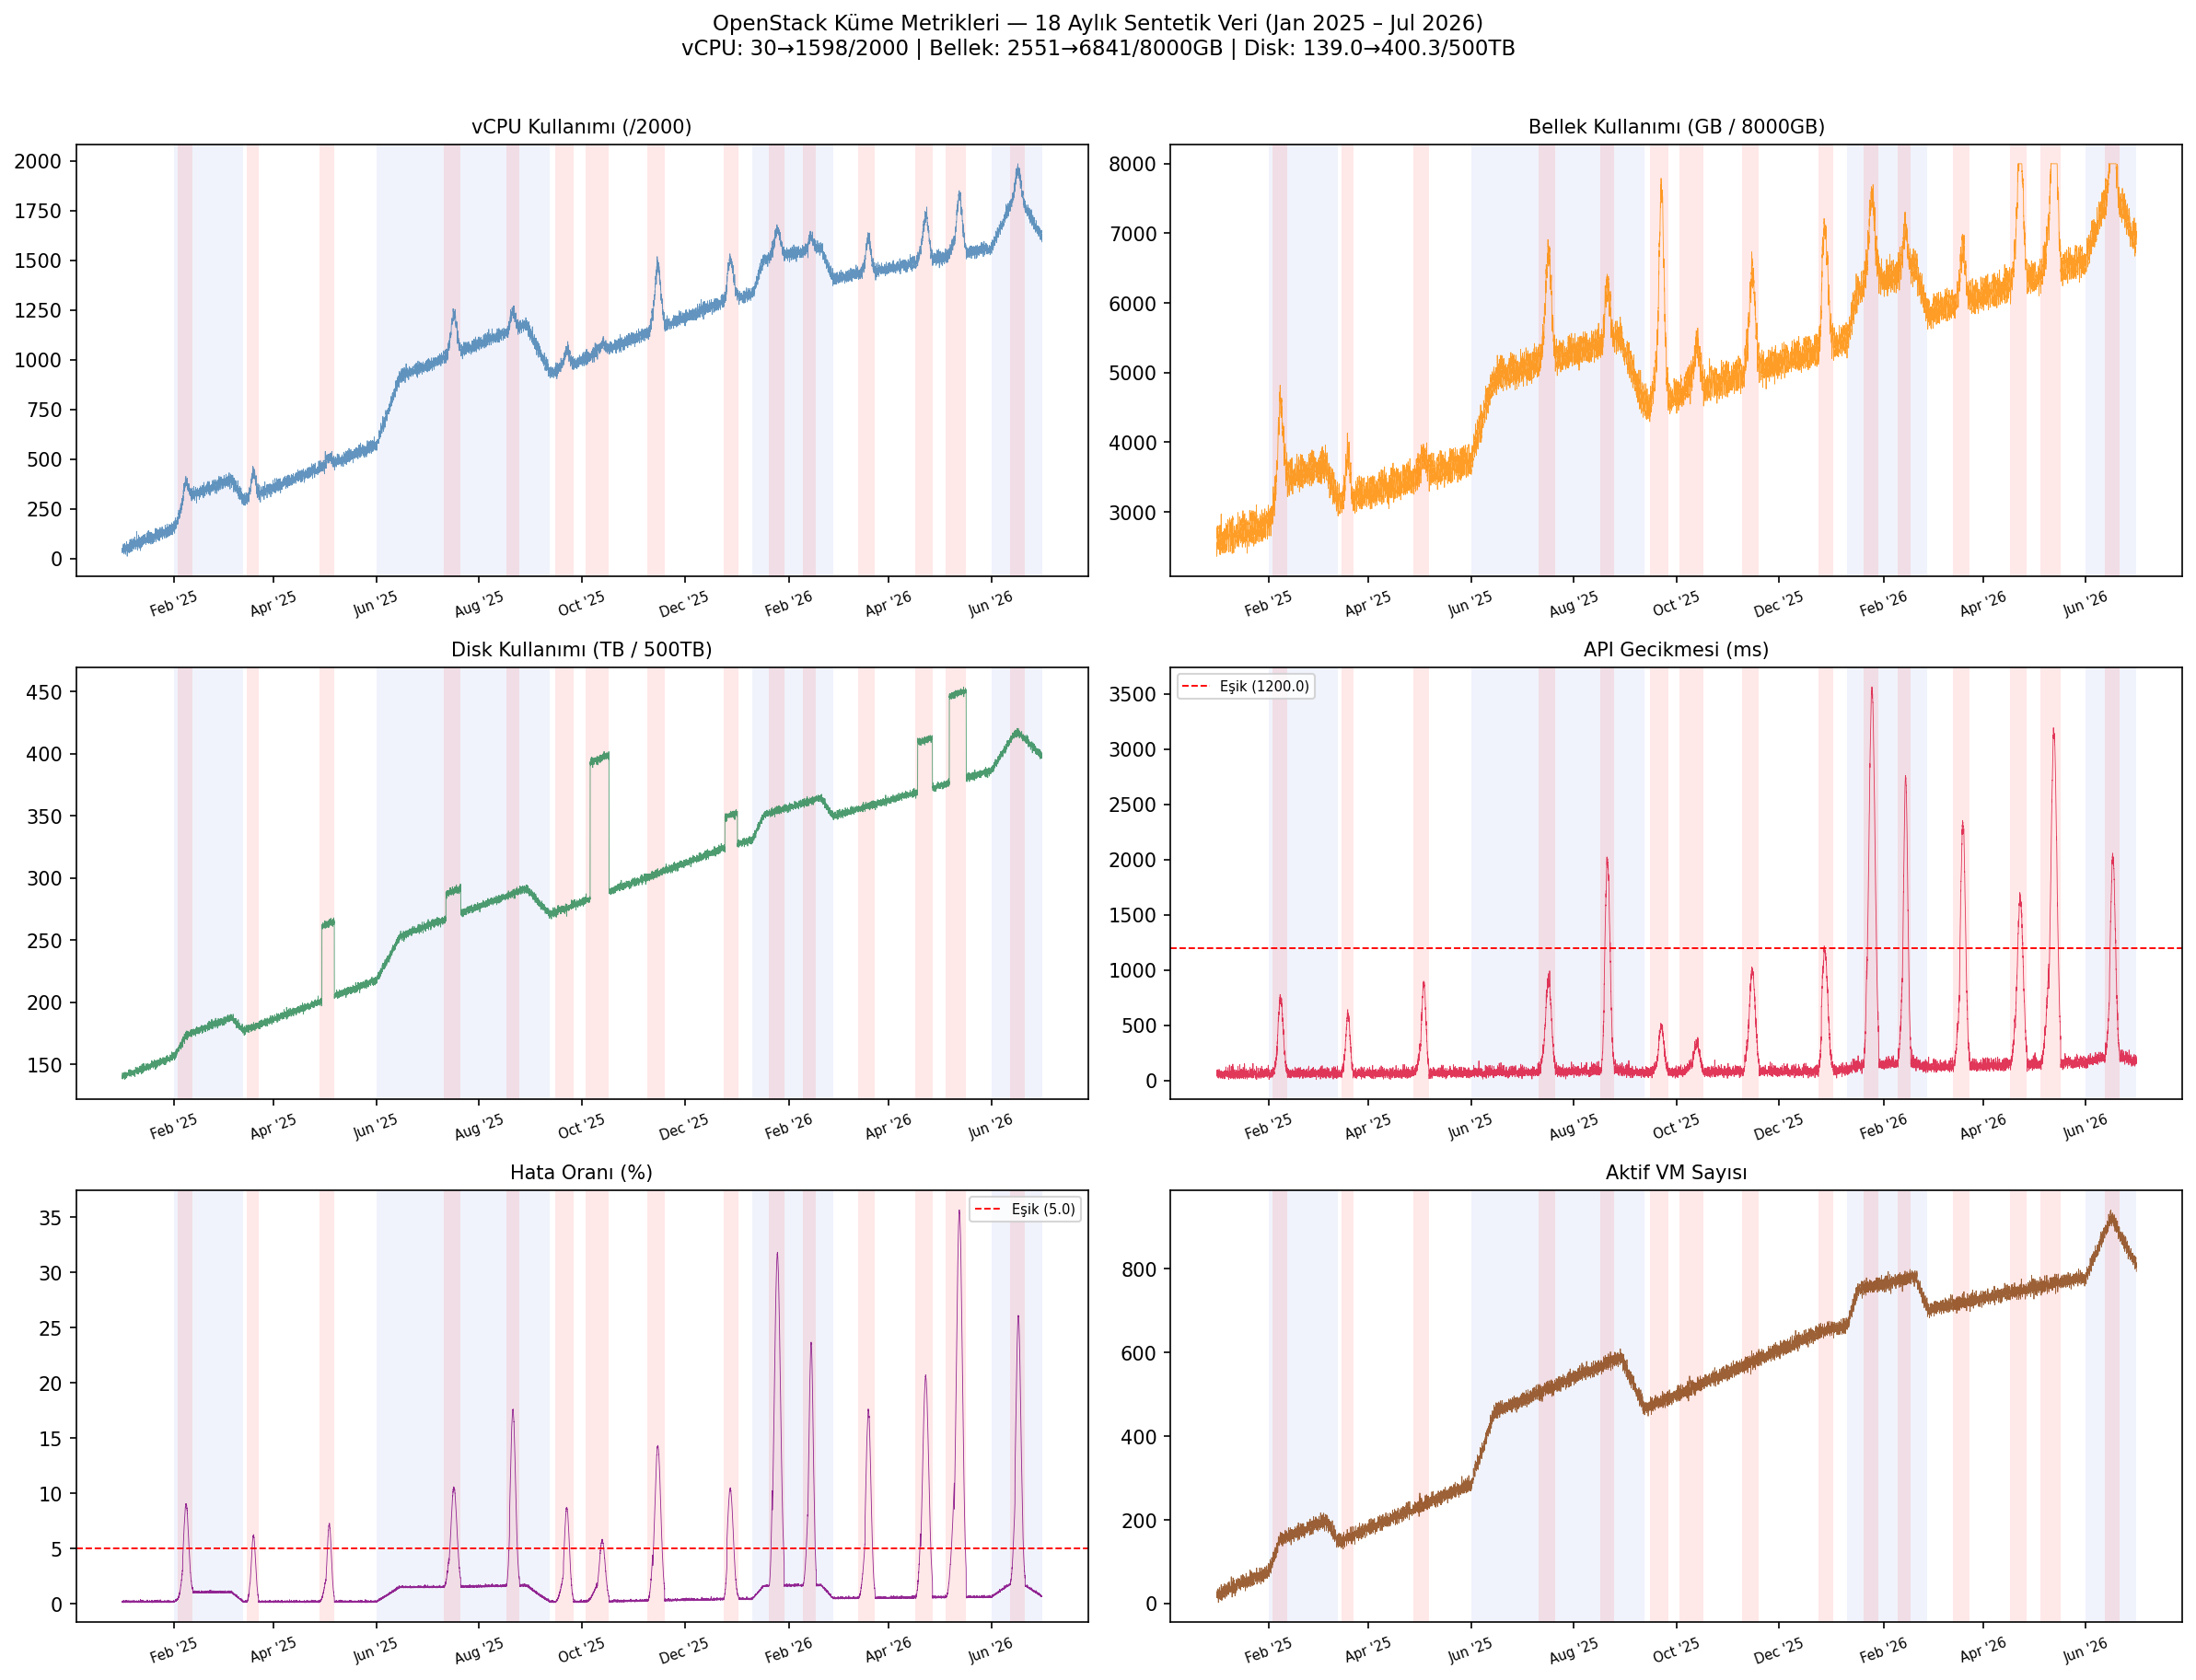
\includegraphics[width=0.92\textwidth]{metrics_overview}
    \caption{CloudMon veri akışı: OpenStack servislerinden metrik (Prometheus/Thanos) ve log (Fluentd/OpenSearch) verilerinin toplanması ve pipeline'a beslenmesi.}
    \label{fig:veriakisi}
\end{figure}


\section{Veri Kümesi}

\subsection{Metrik Verisi}

Metrik verisi, OpenStack Nova (işlem), Cinder (depolama) ve Neutron (ağ) bileşenlerinden Prometheus/Thanos aracılığıyla saatlik aralıklarla toplanmıştır.
Veri kümesi Ocak 2025 -- Temmuz 2026 dönemini kapsayan 18 aylık bir zaman aralığına karşılık gelmekte ve toplam 13.104 saatlik gözlem noktası içermektedir.

Birincil kaynak değişkenleri \autoref{tab:metrikler}'de özetlenmektedir.

\begin{table}[htbp]
    \centering
    \caption{Kullanılan metrik değişkenleri}
    \label{tab:metrikler}
    \begin{tabular}{lll}
        \textbf{Değişken} & \textbf{Açıklama} & \textbf{Birim} \\
        \hline
        \texttt{vcpu\_usage\_percent}   & vCPU tahsis oranı      & \% \\
        \texttt{memory\_usage\_percent} & Bellek kullanım oranı  & \% \\
        \texttt{disk\_usage\_percent}   & Disk kullanım oranı    & \% \\
        \texttt{api\_latency\_ms}       & API yanıt gecikmesi    & ms \\
        \texttt{error\_rate\_percent}   & Hata oranı             & \% \\
        \texttt{network\_in\_mbps}      & Gelen ağ trafiği       & Mbps \\
        \texttt{network\_out\_mbps}     & Giden ağ trafiği       & Mbps \\
        \texttt{api\_requests\_per\_hour} & Saatlik API istek sayısı & adet/saat \\
        \texttt{vm\_count}              & Aktif sanal makine sayısı & adet \\
    \end{tabular}
\end{table}

\subsection{Log Verisi}

Log verisi, OpenSearch'te depolanan OpenStack servis loglarından saatlik pencere bazında sayım olarak türetilmiştir.
Log tipleri iki kategoriye ayrılmaktadır:

\textbf{Hata logları} (8 tip): \texttt{timeout}, \texttt{db\_connection}, \texttt{resource\_exhausted}, \texttt{quota\_exceeded}, \texttt{auth\_failure}, \texttt{network\_error}, \texttt{scheduler\_error}, \texttt{io\_error}.

\textbf{Erken uyarı logları} (7 tip): \texttt{slow\_response}, \texttt{memory\_pressure}, \texttt{connection\_pool\_warn}, \texttt{scheduler\_degradation}, \texttt{quota\_pressure}, \texttt{disk\_io\_degradation}, \texttt{cascade\_indicator}.

Erken uyarı logları hata statüsüne ulaşmamış ancak sistem degradasyonuna işaret eden ön-arıza sinyallerini temsil etmektedir.

\subsection{Eğitim ve Test Bölünmesi}

Zaman serisi veri setinde bilgi sızıntısını (data leakage) önlemek amacıyla sabit kesim noktası yöntemi kullanılmıştır.
Ocak 2025 -- Mart 2026 arası 15 aylık dönem eğitim kümesini, Nisan 2026 -- Haziran 2026 arası 3 aylık dönem ise test kümesini oluşturmaktadır.
Bu bölünme yaklaşık \%83 eğitim -- \%17 test oranına karşılık gelmektedir.


\section{Log İşleme Pipeline'ı}
\label{sec:logpipeline}

Ham log sayımlarından operasyonel içgörülere ulaşmak amacıyla dört aşamalı bir pipeline tasarlanmıştır.
Pipeline çıktısı \autoref{fig:logpipeline}'de görselleştirilmektedir.

\begin{figure}[htbp]
    \centering
    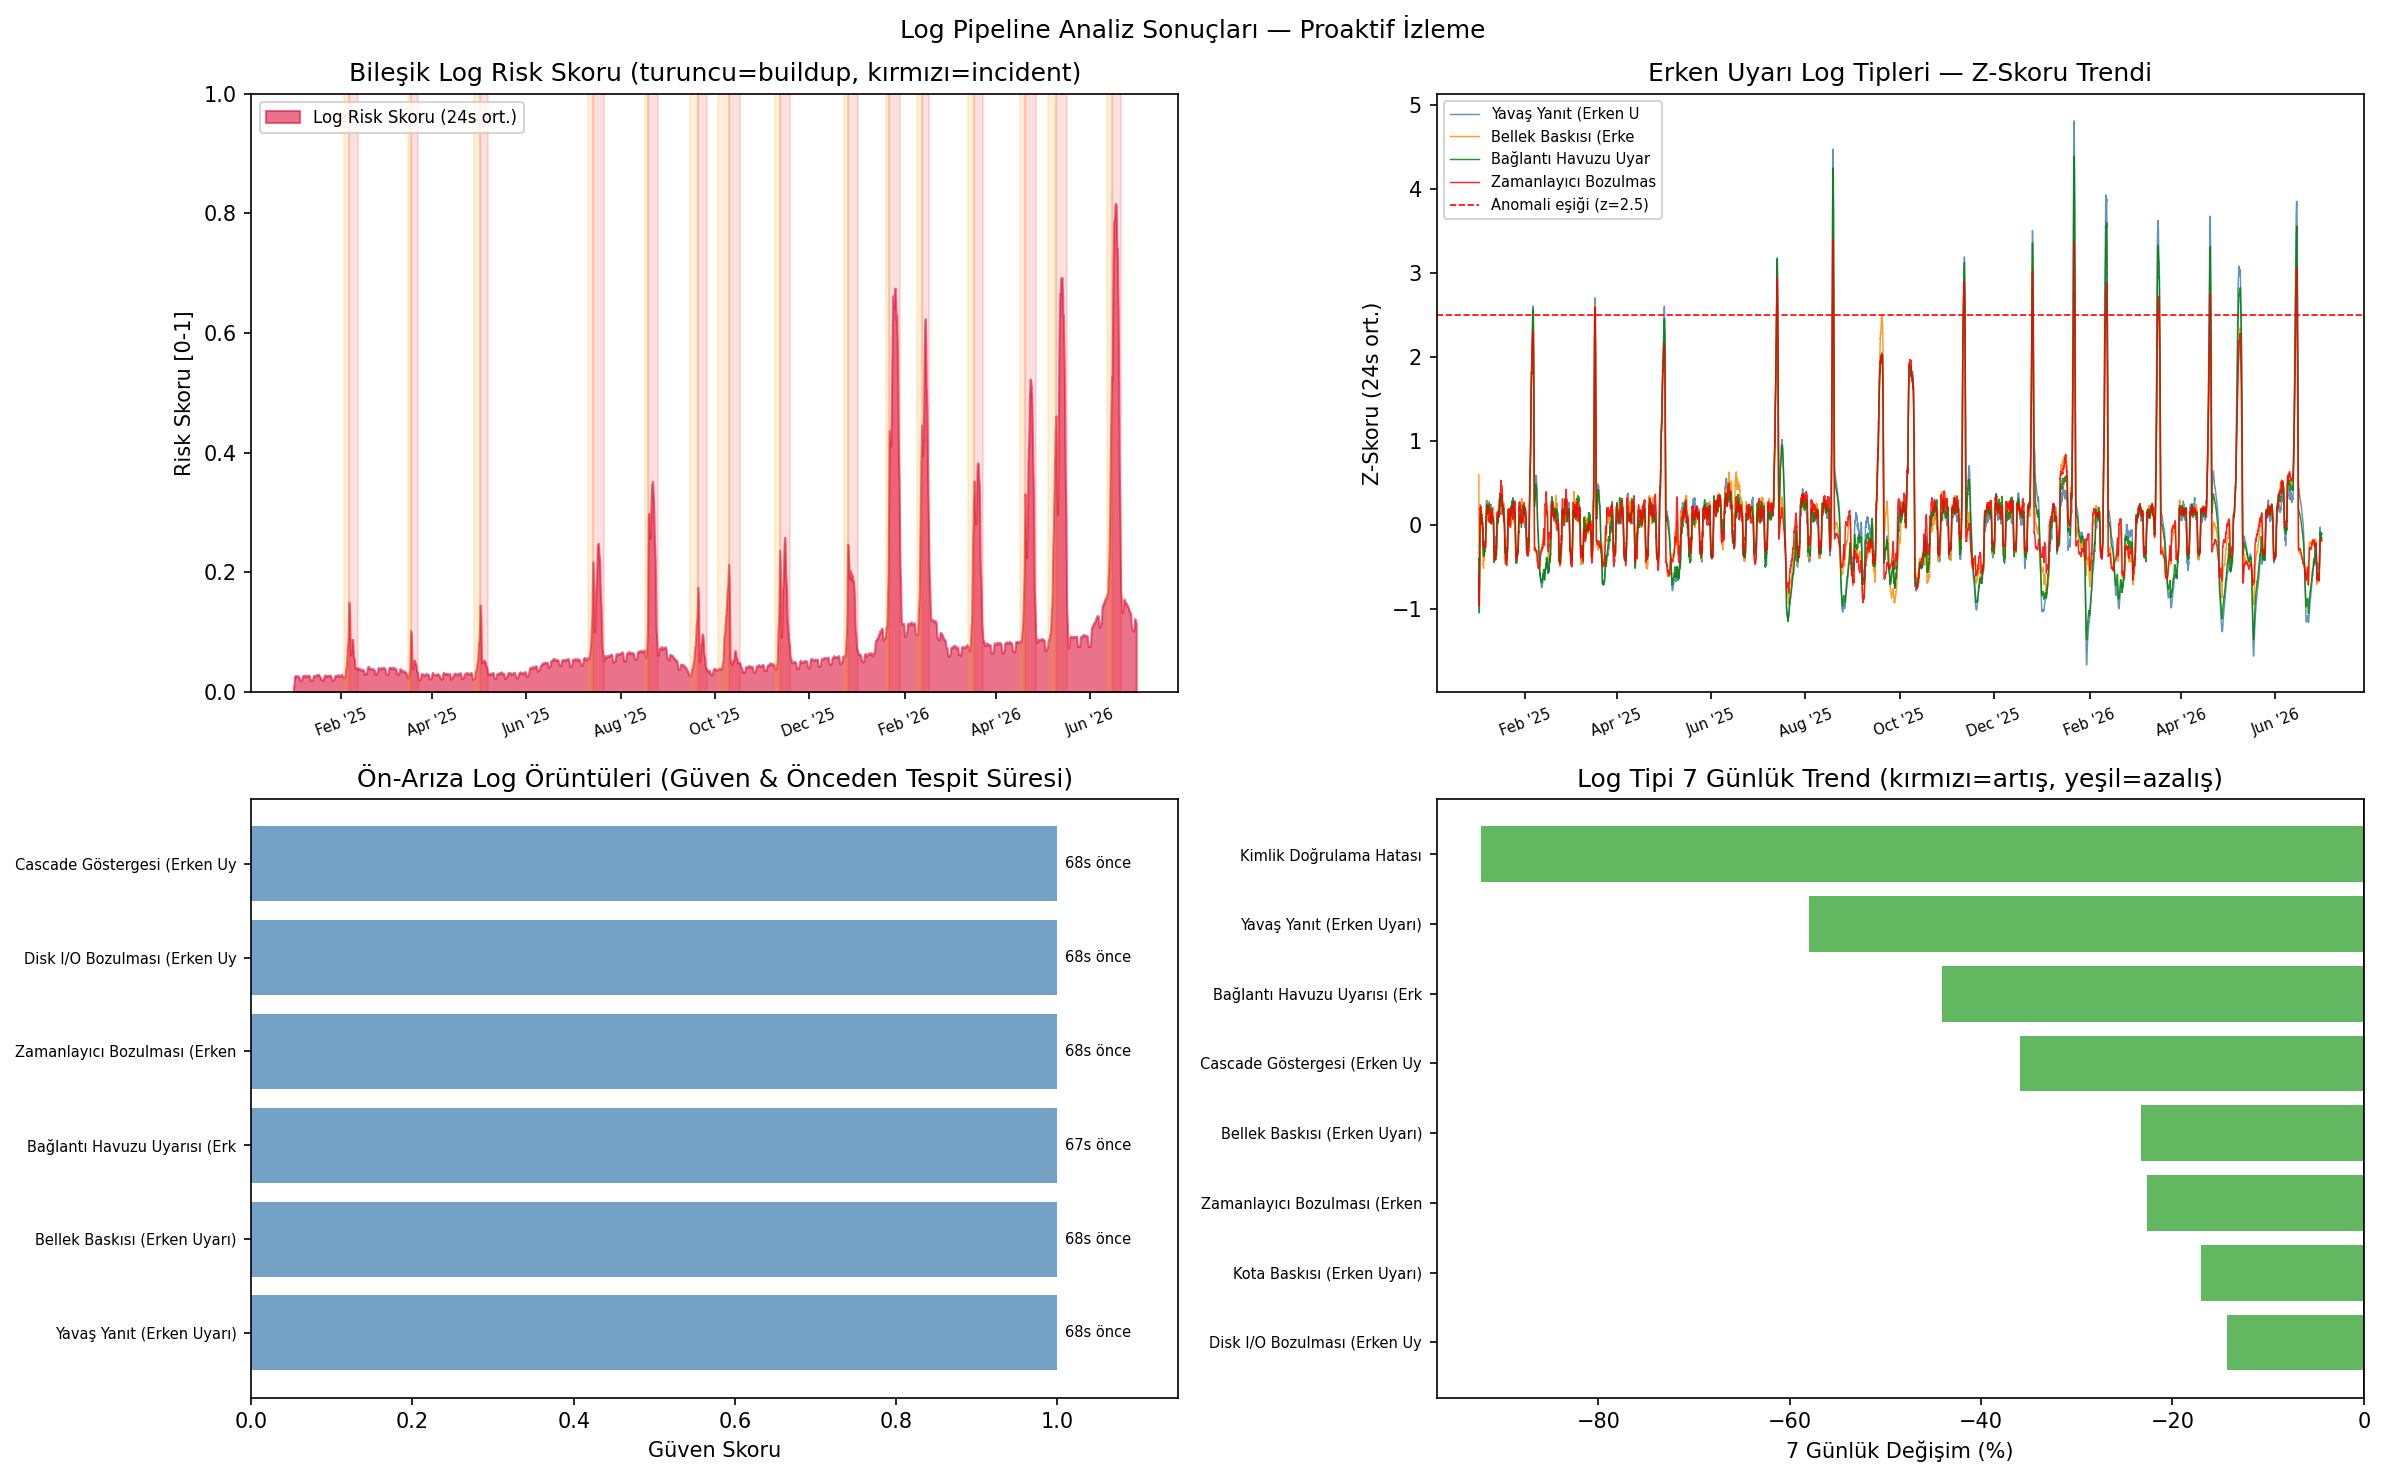
\includegraphics[width=0.90\textwidth]{log_pipeline_analysis}
    \caption{Dört aşamalı log işleme pipeline'ı çıktıları: log trendi, anomali tespiti ve cascade analizi.}
    \label{fig:logpipeline}
\end{figure}

\subsection{Aşama 1 — Ayrıştırma ve Sınıflandırma}

Bu aşamada ham log sayımları Nova, Neutron, Cinder ve Keystone servisleri bazında servis sağlık skorlarına dönüştürülmekte; erken uyarı ve hata logları ayrı ayrı değerlendirilmektedir.

Her servis için normalize hata skoru $s_j \in [0, 1]$ hesaplanmaktadır:
\begin{equation}
    s_j = \min\!\left(\frac{n_j}{q_{99}(n_j) + \epsilon},\; 1\right)
    \label{eq:servis-skor}
\end{equation}
burada $n_j$ servis $j$'nin saatlik hata sayısını, $q_{99}$ \%99'luk dilimi ve $\epsilon$ sıfıra bölmeyi önleyen küçük bir sabiti temsil etmektedir.

Bileşik log risk skoru ise erken uyarı ve hata bileşenlerinin ağırlıklı toplamı olarak tanımlanmaktadır:
\begin{equation}
    r_{\text{log}} = 0{,}4 \cdot s_{\text{uyarı}} + 0{,}6 \cdot s_{\text{hata}}
    \label{eq:log-risk}
\end{equation}
Ağırlıklar; erken uyarı sinyallerinin yüksek hacimli ama düşük öncelikli, hata loglarının ise düşük hacimli ama yüksek öncelikli olduğu kabulünü yansıtmaktadır.
$r_{\text{log}} \in [0, 1]$ aralığında normalize edilmektedir.

Eşiği aşan servisler ($s_j > 0{,}7$: \textit{degraded}; $s_j > 0{,}9$: \textit{critical}) olarak işaretlenmekte ve bu sınıflandırma cascade risk tespitinde (Aşama 3) kullanılmaktadır.

\subsection{Aşama 2 — Zamansal Agregasyon ve Trend Analizi}

Saatlik log sayımlarından 6, 24 ve 72 saatlik hareketli ortalamalar hesaplanmaktadır.
Her log tipi için 7 günlük pencerede z-skor tabanlı trend yönü (\textit{increasing}, \textit{decreasing}, \textit{stable}) belirlenmektedir.

\subsection{Aşama 3 — Anomali Tespiti}

Z-skor eşiği ($\sigma > 2{,}5$) ve ani artış tespiti (spike detection) ile anormal log yoğunlaşmaları belirlenmektedir.
Birden fazla servisin aynı zaman penceresinde degradasyon göstermesi \textit{cascade} riski olarak işaretlenmekte ve zaman damgası kaydedilmektedir.

\subsection{Aşama 4 — Ön-Arıza Örüntü Çıkarımı}

Geçmiş incident'lerin öncesindeki log imzaları bu aşamada çıkarılmaktadır.
Her log tipi için "arızadan kaç saat önce, ne oranda artış gösterdi?" sorusu yanıtlanmaktadır.
Bu örüntüler hem öneri motoruna hem de LLM'e zenginleştirilmiş bağlam olarak beslenmektedir.
Örneğin \textit{slow\_response} log tipi, geçmiş 15 incident'te arızadan ortalama 68 saat önce \%287 artış göstermiştir.


\section{Özellik Mühendisliği}
\label{sec:ozellik}

Metrik ve log verilerinden toplam 272 özellik türetilmektedir.
Bu özellikler altı kategoride sınıflandırılmaktadır:

\begin{table}[htbp]
    \centering
    \caption{Özellik kategorileri ve sayıları}
    \label{tab:ozellikler}
    \begin{tabular}{lll}
        \textbf{Kategori} & \textbf{Tanım} & \textbf{Örnek} \\
        \hline
        Zaman özellikleri      & Saat, gün, hafta, iş günü & \texttt{hour\_of\_day}, \texttt{is\_weekend} \\
        Hareketli ortalama     & 3/6/12/24/168s pencere & \texttt{vcpu\_rmean\_24h} \\
        Hareketli std.         & 3/6/12/24s pencere     & \texttt{vcpu\_rstd\_24h} \\
        Gecikme (lag)          & 1/6/24/48/168s geri    & \texttt{vcpu\_lag\_24h} \\
        Değişim hızı (delta)   & 1/6/24s fark           & \texttt{vcpu\_delta\_6h} \\
        Log hareketli toplamlari & 6/24/72s pencere    & \texttt{slow\_response\_rsum\_72h} \\
    \end{tabular}
\end{table}

Bunlara ek olarak \texttt{early\_warning\_composite} adlı bir bileşik sinyal hesaplanmaktadır.
Bu sinyal, yedi erken uyarı log tipinin saatlik toplamlarını birleştiren ve genel sistem stresini tek bir boyuta indirgeyen bir özet göstergedir.

Hedef değişken her $h \in \{24, 72\}$ saat ufku için üç kaynak ($\hat{y}$: vCPU, Bellek, Disk kullanım yüzdesi) bazında ayrı ayrı oluşturulmaktadır:
\begin{equation}
    \hat{y}_{t+h} = f(\mathbf{x}_t)
\end{equation}
burada $\mathbf{x}_t$ $t$ anındaki 272 boyutlu özellik vektörünü, $f(\cdot)$ ise eğitilen regresyon modelini temsil etmektedir.


\section{Kapasite Tahmin Modelleri}
\label{sec:modeller}

Her (kaynak, ufuk) çifti için yedi farklı algoritma eğitilmekte; böylece $3 \times 2 \times 7 = 42$ model değerlendirilmektedir:

\begin{enumerate}
    \item Doğrusal Regresyon (LR)
    \item Rastgele Orman (RF)
    \item Gradyan Artırmalı Ağaçlar (GBT)
    \item XGBoost (XGB)
    \item LightGBM (LGBM)
    \item CatBoost
    \item Çok Katmanlı Algılayıcı (MLP)
\end{enumerate}

LR ve MLP modelleri için StandardScaler uygulanmaktadır; ağaç tabanlı modeller (RF, GBT, XGB, LGBM, CatBoost) normalizasyon gerektirmemektedir.
Model hiperparametreleri \autoref{tab:hiperparametre}'de özetlenmektedir.

\begin{table}[htbp]
    \centering
    \caption{Kapasite tahmin modelleri hiperparametreleri}
    \label{tab:hiperparametre}
    \begin{tabular}{lll}
        \textbf{Model} & \textbf{Temel Hiperparametreler} & \textbf{Ön İşleme} \\
        \hline
        Doğrusal Regresyon & — (varsayılan) & StandardScaler \\
        Rastgele Orman     & \texttt{n\_est=200, max\_depth=12, min\_leaf=4} & — \\
        Gradyan Artırmalı  & \texttt{n\_est=200, depth=5, lr=0.08, sub=0.85} & — \\
        XGBoost            & \texttt{n\_est=200, depth=5, lr=0.08, sub=0.85} & — \\
        LightGBM           & \texttt{n\_est=200, depth=5, lr=0.08, sub=0.85} & — \\
        CatBoost           & \texttt{iter=200, depth=5, lr=0.08, sub=0.85}   & — \\
        MLP                & \texttt{layers=(128,64), relu, max\_iter=500, early\_stop} & StandardScaler \\
    \end{tabular}
\end{table}

Tüm ağaç tabanlı modellerde \texttt{random\_state=42} sabitlenmiş; tekrarlanabilirlik sağlanmıştır.
MLP'de erken durdurma (early stopping) ile aşırı öğrenme önlenmektedir.

Tüm modeller yinelemeli tahmin (iterative forecasting) stratejisiyle değerlendirilmektedir.
Her test noktasında yalnızca o ana kadar gözlemlenen veri kullanılmakta; böylece gerçek zamanlı operasyonel kullanım koşulları simüle edilmektedir.


\section{SHAP Açıklanabilirlik Analizi}
\label{sec:shap}

\subsection{Neden SHAP?}

Makine öğrenmesi modelleri, özellikle ağaç tabanlı yöntemler, yüksek tahmin başarısı sunmakla birlikte \textit{kara kutu} niteliği taşımaktadır: model neden bu tahmini yaptı sorusunun cevabı doğrudan elde edilememektedir.
Bulut operasyonu bağlamında bu durum ciddi bir güven sorununa yol açmaktadır; bir operatör ``vCPU kullanımı 74 gün içinde eşiği aşacak'' uyarısını aldığında, bu uyarının arkasındaki sinyali anlayamazsa gerekli aksiyonu almakta tereddüt edebilir.

Geleneksel özellik önem yöntemleri bu sorunu yalnızca kısmen çözebilmektedir.
Karar ağaçlarının Gini önem ölçütü yüksek kardinaliteli özelliklere sistematik olarak daha yüksek puan vermekte ve özellikler arası korelasyonu göz ardı etmektedir \autocite{breiman2001}.
Permütasyon önemi ise özelliğin tahmine katkısının yönünü vermemektedir; bir özelliğin yüksek permütasyon skoru tahmini iyileştirdiğini mi yoksa stabilize ettiğini mi gösterdiği belirsiz kalmaktadır.

SHAP (SHapley Additive exPlanations), kooperatif oyun teorisindeki Shapley değerlerini makine öğrenmesine uyarlayan, teorik olarak temellendirilen bir açıklanabilirlik çerçevesidir \autocite{lundberg2017}.
Her özellik için hesaplanan $\phi_i$ değeri şu garantiyi taşımaktadır: tüm özellik atıf değerlerinin toplamı modelin tahmini ile referans değer (eğitim seti ortalaması) arasındaki farka tam olarak eşittir.
Bu toplamlanabilirlik (additivity) özelliği sayesinde SHAP, ``bu özellik tahmini ne kadar ve hangi yönde etkiledi'' sorusunu tutarlı biçimde yanıtlamaktadır \autocite{lundberg2020}.

CloudMon bu çerçeveyi iki temel amaç için kullanmaktadır.
Birincisi, 272 özellikli yüksek boyutlu uzayda hangi metrik ve log özelliklerinin tahmine gerçekten katkı yaptığını saptamak; böylece hibrit özellik uzayının faydası nicel olarak ölçülmektedir.
İkincisi, her kapasite uyarısına ``en etkili özellik: \texttt{vm\_count\_rmean\_24h}'' biçiminde bir açıklama eklemek ve bu açıklamayı LLM katmanına iletmek; böylece hem operatöre hem de dile dayalı öneri motoruna bağlam sağlanmaktadır.

\subsection{Teknik Uygulama}

Her eğitilmiş model için model tipine uygun SHAP açıklayıcısı seçilmektedir: RF, GBT, XGB, LGBM ve CatBoost için TreeSHAP, LR için LinearExplainer, MLP için KernelSHAP kullanılmaktadır \autocite{lundberg2017, lundberg2020}.
Bu seçim, her yöntem için teorik geçerlilik koşullarını karşılamaktadır; TreeSHAP ağaç yapılarını verimli biçimde gezer, LinearExplainer doğrusal modellerde analitik çözüm üretir.

Üç tür görselleştirme üretilmektedir:
\begin{maddelendir}[label=--]
    \item \textbf{Bar grafiği:} tüm test gözlemlerinde ortalama $|\phi_i|$ ile global özellik önem sıralaması.
    \item \textbf{Beeswarm grafiği:} her gözlem için $\phi_i$ değerinin dağılımı ve özellik değeriyle renk kodlaması; hem global hem de yerel örüntüleri görselleştirir.
    \item \textbf{Bağımlılık grafiği:} seçili bir özelliğin değeri ile SHAP katkısı arasındaki ilişki; doğrusal olmayan etkileri ortaya koymaktadır.
\end{maddelendir}

vCPU tahmininde elde edilen bar grafiği \autoref{fig:shap-bar-vcpu}'da verilmektedir.

\begin{figure}[htbp]
    \centering
    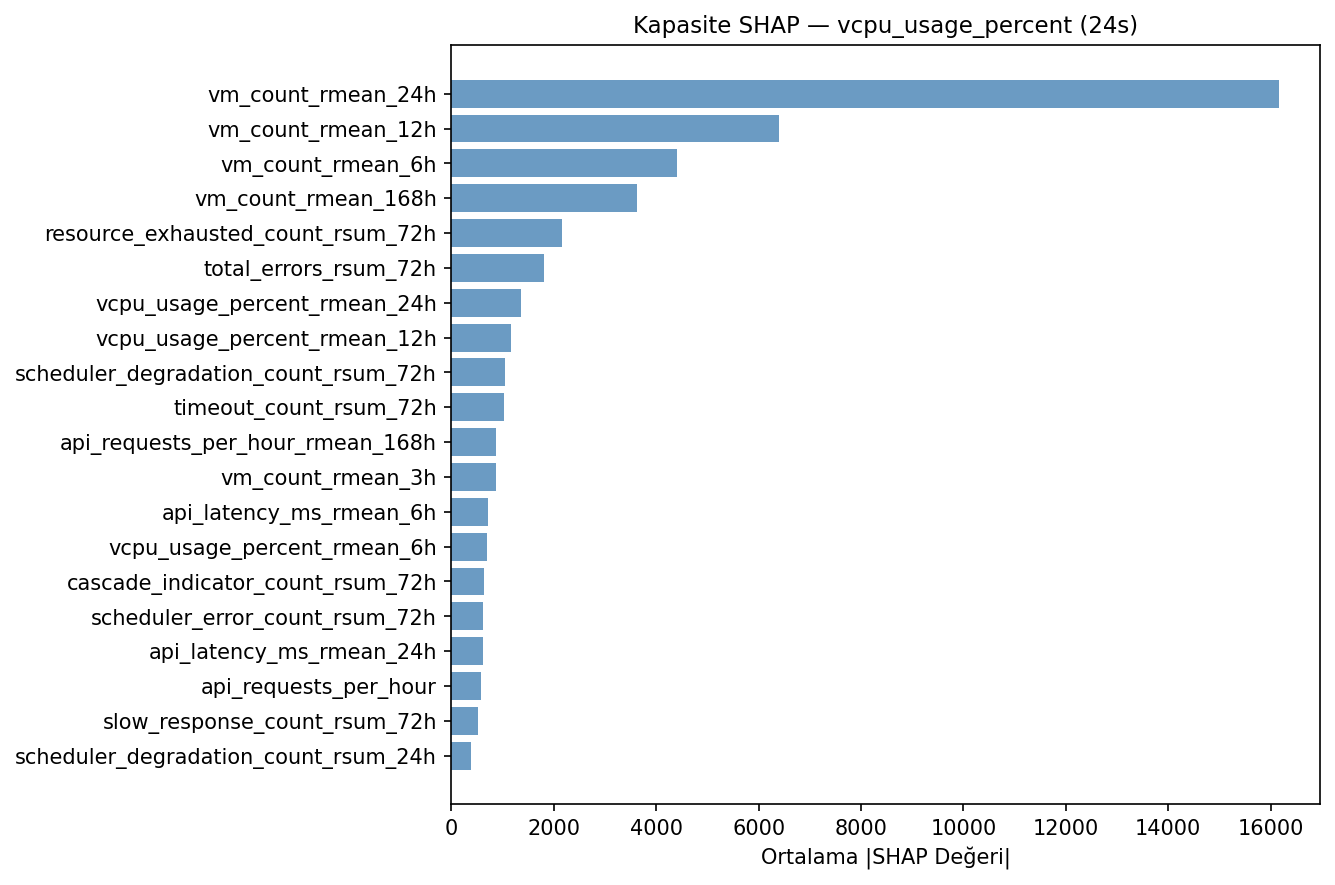
\includegraphics[width=0.85\textwidth]{shap_capacity_bar_vcpu_usage_percent_24h}
    \caption{vCPU 24 saatlik tahmin modeli için SHAP özellik önem sıralaması (ilk 20 özellik).}
    \label{fig:shap-bar-vcpu}
\end{figure}


\section{Öneri Motoru ve LLM Entegrasyonu}
\label{sec:oneri}

\subsection{Neden LLM?}

Kural tabanlı sistemler, eşik aşımlarını ve log anomalilerini güvenilir biçimde tespit eder; ancak bu sinyalleri birleştirerek operatörün ne yapması gerektiğini söyleyemez.
Gerçek bir bulut ortamında aynı anda onlarca uyarı tetiklenebilir: bellek eşiğine yaklaşma, kota aşımı log artışı, zamanlayıcı bozulma ve üç servisin eş zamanlı degradasyonu birbirinden bağımsız alarm olarak göründüğünde, operatör önce hangisine müdahale edeceğine kendi deneyimiyle karar vermek zorunda kalır.

Büyük Dil Modelleri (BDM/LLM), yapılandırılmış bağlam verildiğinde bu sentezi doğal dil akıl yürütmesiyle gerçekleştirebilmektedir.
LLM, hem sayısal verileri (kullanım oranı, z-skoru, tahmini gün sayısı) hem de niteliksel sinyalleri (SHAP sıralaması, ön-arıza örüntüsü, cascade riski) birden okuyan bir uzman gibi davranmakta; bunları önceliklendirilmiş ve gerekçelendirilmiş aksiyon önerilerine dönüştürmektedir \autocite{brown2020, openai2023, anthropic2024}.

CloudMon'da LLM katmanının iki kritik işlevi vardır.
Birincisi, kural motorunun ürettiği ayrı uyarıları tek bir tutarlı operasyonel rapora sentezlemek; ikincisi, SHAP'ın sağladığı ``en etkili özellik'' açıklamasını doğal dil bağlamına taşıyarak operatörün tahminin \textit{neden} yapıldığını anlamasını sağlamaktır.
Bu yaklaşım, CloudMon'u salt bir izleme aracından açıklanabilir ve eyleme dönüştürülebilir bir karar destek sistemine dönüştürmektedir.

\subsection{Neden Zenginleştirilmiş Bağlam?}

LLM performansı, aldığı bağlamın kalitesiyle doğrudan ilişkilidir.
Ham metrik sayıları (``vCPU \%79{,}6, Bellek \%85{,}5'') tek başına bir operasyonel değer taşımaz; modelin bu sayılardan eyleme dönüştürülebilir bir öneri çıkarabilmesi için trendin yönü, beklenen eşik tarihi, log örüntüleri ve SHAP açıklaması gibi bağlam katmanlarına ihtiyacı vardır.
Bu nedenle CloudMon, LLM'e gönderilen istemde şu bilgi katmanlarını birleştirmektedir:

\begin{maddelendir}[label=--]
    \item Kapasite durumu: mevcut kullanım oranı, eşik değeri, trend ve tahmini aşım tarihi
    \item SHAP özellik sıralaması: tahmine en çok katkı yapan metrik veya log tipi (operatörün müdahale noktasını belirlemesi için)
    \item Log anomali özeti: z-skor eşiklerini aşan log tipleri ve yüzdesel artış değerleri
    \item Ön-arıza örüntüsü: geçmiş incident imzalarıyla örtüşen güncel log artışları ve tarihsel öncü süre
    \item Cascade risk bilgisi: eş zamanlı degradasyon gösteren servisler
    \item Servis sağlık durumu: her OpenStack servisinin anlık durum özeti
\end{maddelendir}

\subsection{Kural Tabanlı Katman}

LLM'e iletilmeden önce kural tabanlı motor dört kanaldan uyarı üretmektedir:
\begin{maddelendir}[label=\arabic*.]
    \item \textbf{Kapasite kanalı:} Kapasite modeli tahminleri ve lineer trend analizi birleştirilmekte; tahmini eşik aşım tarihi hesaplanmaktadır. vCPU için $+0{,}275\%$/gün artış trendi ve \%90 eşiği göz önüne alındığında tahmini eşik tarihi çalışma zamanında dinamik olarak belirlenmektedir.
    \item \textbf{Log anomali kanalı:} Z-skor eşiğini ($\sigma > 2{,}5$) aşan log tiplerinde uyarı üretilmektedir.
    \item \textbf{Ön-arıza örüntü kanalı:} Aşama 4'te çıkarılan geçmiş arıza imzalarıyla örtüşen güncel log örüntüleri tespit edilmektedir.
    \item \textbf{Cascade risk kanalı:} Birden fazla servisin eş zamanlı degradasyonu cascade uyarısı olarak raporlanmaktadır.
\end{maddelendir}

\subsection{LLM Katmanı}

Kural tabanlı katmanın çıktıları yukarıda listelenen bağlam katmanlarıyla birleştirilerek yapılandırılmış bir istem oluşturulmaktadır.
Bu istem Claude Sonnet (\texttt{claude-sonnet-4-6}) ve GPT-4o (\texttt{gpt-4o}) modellerine paralel olarak iletilmektedir.
Her iki modelin yanıtı tek bir operasyonel rapora derlenmekte; KRİTİK / UYARI öncelik sıralaması ve servis bazında somut aksiyon önerileri içermektedir.
API anahtarı yapılandırılmadığında sistem, kural tabanlı katmanın çıktılarını doğrudan raporlamakta; LLM sentez katmanı devre dışı kalmaktadır.

% TODO: Bulgular bölümü — CloudMon deney sonuçları
% - 42 model karşılaştırma tabloları (vCPU, Bellek, Disk × 24h, 72h)
% - SHAP özellik önem grafikleri
% - Log anomali tespiti sonuçları
% - Öneri motoru çıktı örnekleri

\chapter{BULGULAR}
\label{ch:bulgular}

Bu bölüm yazılacak.

\chapter{SONUÇLAR VE ÖNERİLER}
\label{ch:sonuclar}

Bu bölümde CloudMon sisteminin deneysel bulgularından çıkarılan sonuçlar özetlenmekte, çalışmanın özgün katkıları değerlendirilmekte ve çalışmanın sınırlılıkları ile gelecek araştırma önerileri tartışılmaktadır.


\section{Temel Bulgular}
\label{sec:sonuc-bulgular}

Bu çalışma; kapasite tahmini, açıklanabilirlik analizi ve log tabanlı erken uyarı olmak üzere üç ana araştırma ekseninde somut bulgular üretmiştir.

\subsection{Kapasite Tahmin Modeli}

42 model (7 algoritma $\times$ 3 kaynak $\times$ 2 ufuk) değerlendirmesinin en belirgin bulgusu, Doğrusal Regresyon'un (LR) ağaç tabanlı tüm algoritmaları geride bırakmasıdır.
24 saatlik ufukta LR, vCPU için R\textsuperscript{2}\,=\,0{,}9577, Bellek için R\textsuperscript{2}\,=\,0{,}7945 ve Disk için R\textsuperscript{2}\,=\,0{,}6984 değerlerine ulaşmıştır.
En yakın rakibi olan Gradyan Artırmalı Ağaçlar, vCPU 24\,s senaryosunda yalnızca R\textsuperscript{2}\,=\,0{,}1079 üretmiştir; bu fark, OpenStack zaman serilerinin test döneminde güçlü monoton trendler barındırdığını ve LR'nin bu trendi gecikme ve hareketli ortalama özellikleri üzerinden doğrudan öğrendiğini göstermektedir.

72 saatlik ufukta sonuçlar kaynak bazında ayrışmaktadır.
vCPU'da LR, R\textsuperscript{2}\,=\,0{,}7728 ile etkin tahmin gücünü korumuştur.
Bellek ve Disk'te ise MLP en iyi performer konumuna geçmiş; bununla birlikte R\textsuperscript{2} değerleri sırasıyla 0{,}3456 ve 0{,}2212'ye gerilemiştir.
Ağaç tabanlı modellerin büyük çoğunluğu 72 saatlik ufuklarda negatif R\textsuperscript{2} üretmiş, yani ortalama tahminden daha kötü performans göstermiştir.
Bu bulgu, söz konusu modellerin 272 özellikli yüksek boyutlu uzayda eğitim kümesine aşırı uyduğunu ve zaman serisi genellemesinde yetersiz kaldığını ortaya koymaktadır.

\subsection{SHAP Açıklanabilirlik Bulguları}

SHAP analizi, log tabanlı özelliklerin salt metrik özelliklerinden anlamlı biçimde farklılaştığını ve kapasite tahminine bağımsız katkı yaptığını nicel olarak göstermiştir.
vCPU 24\,s modelinin ilk 10 özelliği arasında dört log özelliği yer almaktadır:
\texttt{resource\_exhausted\_count\_rsum\_72h} (5.\ sıra, $|\phi|$\,=\,2\,150),
\texttt{total\_errors\_rsum\_72h} (6.\ sıra, $|\phi|$\,=\,1\,800),
\texttt{scheduler\_degradation\_count\_rsum\_72h} (9.\ sıra, $|\phi|$\,=\,1\,050) ve
\texttt{timeout\_count\_rsum\_72h} (10.\ sıra, $|\phi|$\,=\,1\,028).
Disk 24\,s modelinde ise \texttt{total\_errors\_rsum\_24h} birinci sıraya taşınmış; log özellikleri metrik özelliklerini bile geride bırakmıştır.
Bu bulgular, log verilerinin kapasite tahmininde salt gürültü değil, anlamlı bir sinyal kaynağı olduğunu kanıtlamakta ve hibrit özellik uzayının kurucu varsayımını doğrulamaktadır.

\subsection{Log Analizi ve Erken Uyarı}

Dört aşamalı log işleme pipeline'ı (trend tespiti, z-skor anomali tespiti, ön-arıza örüntü eşleştirme, cascade risk tespiti) test dönemi (Nisan--Haziran 2026) üzerinde anlamlı sinyaller üretmiştir.
\textit{Slow\_response} loglarının geçmiş 15 incident analizine göre arızadan ortalama 68 saat önce \%287 oranında artış gösterdiği bulunmuş ve mevcut test dönemi verisi bu örüntüyle örtüşmüştür.
Kota aşımı loglarının z-skoru 4{,}5'e çıkmış; disk I/O hatası (z\,=\,3{,}6), ağ hatası (z\,=\,2{,}8) ve veritabanı bağlantı hatası (z\,=\,2{,}6) da anormallik eşiğini (\,$\sigma > 2{,}5$) aşmıştır.
2026-06-28 tarihinde Nova, Neutron ve Keystone servislerinin eş zamanlı degradasyonu cascade risk kanalı tarafından tespit edilmiştir.
Bu bulgular, log tabanlı erken uyarı mekanizmasının metrik eşik alarmlarına kıyasla üç güne yakın önceden sinyal üretme potansiyeline sahip olduğunu göstermektedir.

\subsection{Öneri Motoru ve LLM Entegrasyonu}

Kural tabanlı motor ve LLM katmanı (Claude Sonnet + GPT-4o) birlikte 9 öneri üretmiştir: 2 KRİTİK ve 7 UYARI.
LLM'e iletilen zenginleştirilmiş bağlam; kapasite durumunu, log anomali özetini, SHAP özellik sıralamasını ve cascade risk skorunu kapsamaktadır.
Üretilen öneriler, tahmin modelinin sayısal çıktısını (tahmini eşik tarihi), SHAP açıklamasını (en etkili özellik) ve log analizini (erken uyarı korelasyonu) somut operasyonel aksiyonlarla birleştirmektedir.
Bu yapı, CloudMon'un reaktif bir izleme aracı olmanın ötesine geçerek açıklanabilir ve eyleme dönüştürülebilir öneriler üreten bir operasyonel zekâ sistemi olduğunu göstermektedir.


\section{Tezin Özgün Katkıları}
\label{sec:sonuc-katkilar}

Bu çalışma, kapsamlı deneysel değerlendirme çerçevesinde aşağıdaki dört özgün katkıyı sunmaktadır:

\begin{enumerate}
    \item \textbf{Log--metrik korelasyonuna dayalı kapasite tahmini:}
    Metrik ve log verilerinin ortak bir özellik uzayında birleştirilmesi, her iki veri kaynağının da kapasite tahminine anlamlı katkı yaptığını göstermiştir.
    SHAP analizi, log tabanlı özelliklerin yalnızca metrik özelliklerini değil, ağaç tabanlı modellerin gördüğü her iki veri tipini de geride bırakabildiğini nicel olarak ortaya koymuştur.
    Hibrit özellik uzayı, yalnızca metrik tabanlı yaklaşımlara kıyasla SHAP ilk 10'unda \%40 log özellik payıyla (vCPU 24\,s) üstün açıklanabilirlik sunmaktadır.

    \item \textbf{Dört aşamalı log işleme pipeline'ı:}
    Ham log sayımlarından ön-arıza örüntü eşleştirmesine ve cascade risk tespitine uzanan sistematik analiz hattı, tek bir aşamalı log sayımı yaklaşımlarına kıyasla daha zengin ve erken sinyaller üretmektedir.
    Ön-arıza örüntüsünün 68 saatlik öncü uyarı özelliği, operasyonel müdahale için pratik bir zaman penceresi sağlamaktadır.

    \item \textbf{Açıklanabilir kapasite tahmin sistemi:}
    Her tahmin için hesaplanan SHAP değerleri; hangi metriğin ya da log tipinin kararı yönlendirdiğini operatöre aktarmaktadır.
    Bu yaklaşım, kara kutu tahmin modellerini yorumlanabilir aksiyon önerilerine dönüştürerek bulut operatörlerinin karara güvenmesini ve gereksiz kota artışı kararlarını daha bilinçli değerlendirmesini sağlamaktadır.

    \item \textbf{Zenginleştirilmiş bağlamla LLM destekli öneri motoru:}
    Kapasite durumu, log anomali sinyalleri, SHAP özellik önem sıralaması ve cascade riski bir araya getirilerek yapılandırılmış bağlam oluşturulmuş; bu bağlam Claude Sonnet ve GPT-4o modellerine iletilmiştir.
    Üretilen öneriler, sayısal tahmin çıktısı ile yorumsal açıklamayı birleştiren servis bazında önceliklendirilmiş aksiyonlar içermekte; böylece operatörün ayrı sistemlere bakma zorunluluğunu ortadan kaldırmaktadır.
\end{enumerate}


\section{Sınırlılıklar}
\label{sec:sonuc-sinirliliklar}

Bu çalışmanın değerlendirilmesinde aşağıdaki sınırlılıklar göz önünde bulundurulmalıdır:

\begin{enumerate}
    \item \textbf{Eğitim kümesi büyüklüğü ve tek küme:}
    Modeller tek bir OpenStack kümesinin yaklaşık 9 aylık verisine (Temmuz 2025--Mart 2026) dayalı olarak eğitilmiştir.
    Bu durum, ağaç tabanlı modellerin zaman serisi genellemesinde başarısız olmasının kısmi nedeni olabilir; daha uzun eğitim veya farklı kümelerden elde edilen veriler ağaç modellerini güçlendirebilir.
    Ayrıca bulgular, yalnızca bu kümenin iş yükü örüntüsü için geçerli olup farklı ölçek veya kullanım biçimlerine sahip OpenStack kümelerine doğrudan genellenemeyebilir.

    \item \textbf{72 saatlik Disk tahmin gücünün sınırlı olması:}
    Disk 72\,s senaryosunda yalnızca MLP pozitif R\textsuperscript{2} (0{,}2212) üretmiş; diğer tüm modeller rassal tahminden daha kötü performans sergilemiştir.
    Disk kullanımının uzun vadede sergilediği düzensiz ve veri bağımlı örüntüsü, mevcut özellik kümesiyle yeterince yakalanamamaktadır.
    Bu tahmin ufku için ek özellik mühendisliği veya daha gelişmiş zaman serisi modelleri gerekmektedir.

    \item \textbf{LLM çıktılarının nesnel değerlendirmesi:}
    Öneri motorunun LLM katmanı, üretilen önerilerin kalitesini nesnel ölçütlerle değerlendirmek için bir insan değerlendirmesi (human evaluation) ya da karşılaştırma taban çizgisi (baseline) kullanılmamıştır.
    Mevcut değerlendirme, üretilen aksiyonların içerik kontrolüne dayanmakta olup operasyonel uygulamada etkinliklerini doğrulayan kontrollü bir deney yapılamamıştır.

    \item \textbf{Gerçek zamanlı pipeline yokluğu:}
    CloudMon, bu çalışma kapsamında toplu (batch) veri işleme ile test edilmiştir.
    Canlı OpenStack ortamında akış verisi işleme (streaming), model güncelleme gecikmesi ve düşük gecikimli öneri üretimi gibi operasyonel zorluklar deneysel ortamda ele alınmamıştır.
\end{enumerate}


\section{Gelecek Çalışma Önerileri}
\label{sec:sonuc-gelecek}

Bu çalışmanın bulguları ve sınırlılıkları ışığında aşağıdaki araştırma yönleri önerilmektedir:

\begin{enumerate}
    \item \textbf{Daha uzun ve çok kümeli veri ile model genellemesi:}
    Ağaç tabanlı modellerin genelleme yetersizliği, birden fazla OpenStack kümesinden toplanan ve birkaç yıllık zaman aralığını kapsayan verilerle yeniden değerlendirilebilir.
    Transfer öğrenme yaklaşımları, bir kümede eğitilen modelin diğer kümelere uyarlanmasını sağlayarak küme-özgü eğitim maliyetini azaltabilir.

    \item \textbf{Artımlı ve çevrimiçi öğrenme:}
    Bulut iş yükleri zamanla değiştiğinden, modellerin yeni gelen verilerle sürekli güncellenmesini sağlayan artımlı öğrenme (incremental learning) ve kavram kayması (concept drift) tespiti mekanizmaları sisteme entegre edilmelidir.
    Bu yaklaşım, modellerin uzun vadeli operasyonel geçerliliğini koruyacaktır.

    \item \textbf{Gerçek zamanlı akış mimarisi:}
    Mevcut toplu işleme pipeline'ı, Apache Kafka veya benzer bir akış platformu üzerine yeniden tasarlanarak düşük gecikmeli uyarı üretimi sağlanabilir.
    Gerçek zamanlı özellik hesaplama, özellikle cascade riski gibi zaman-kritik uyarıların pratikte değer üretmesini mümkün kılacaktır.

    \item \textbf{LLM çıktılarının kontrollü değerlendirmesi:}
    Öneri motorunun etkinliği, bulut operatörlerinin katılımıyla yürütülecek bir kullanıcı çalışmasıyla ölçülebilir.
    Bu çalışma; üretilen önerilerin doğruluğunu, uygulanabilirliğini ve operatör güvenini nicel olarak değerlendirme olanağı sunacaktır.
    Ayrıca farklı LLM modelleri (açık kaynak ile kapalı kaynak) karşılaştırmalı olarak test edilebilir.

    \item \textbf{Disk 72 saatlik tahmin için gelişmiş yöntemler:}
    Disk kullanımının uzun vadeli örüntüsünü daha iyi yakalamak amacıyla ayrıştırma tabanlı modeller (STL, Prophet) veya LSTM gibi dizi tabanlı derin öğrenme mimarileri araştırılabilir.
    Ayrıca I/O olaylarına dayalı olay güdümlü (event-driven) özellikler, bu senaryodaki tahmin boşluğunu kapatabilir.

    \item \textbf{Diğer bulut platformlarına genişleme:}
    CloudMon mimarisinin AWS, Azure veya Kubernetes kümelerine uyarlanması, platform bağımsız bir AIOps çerçevesi geliştirme ve farklı altyapı örüntülerinde bulguların tekrarlanabilirliğini test etme açısından değerli bir araştırma yönü oluşturmaktadır.
\end{enumerate}


\section{Genel Değerlendirme}

Bu tez, OpenStack tabanlı özel bulut altyapılarında proaktif kapasite yönetimini desteklemeye yönelik uçtan uca bir AIOps sistemi olan CloudMon'u tanıtmış ve deneysel olarak değerlendirmiştir.
Hibrit özellik mühendisliği, açıklanabilir makine öğrenmesi ve LLM tabanlı öneri üretimini entegre eden bu yaklaşım; mevcut literatürdeki izole çalışmaların ötesine geçerek birden fazla analiz katmanını tek bir operasyonel zekâ platformunda bir araya getirmektedir.

Deneysel bulgular, Doğrusal Regresyon'un 24 saatlik ufuklarda ağaç tabanlı modellere kıyasla belirgin biçimde üstün olduğunu; log özelliklerinin SHAP analizinde güçlü bir sinyal kaynağı oluşturduğunu ve dört aşamalı log pipeline'ının metrik eşik alarmlarına üç güne yakın zaman önünde uyarı üretme kapasitesine sahip olduğunu göstermiştir.
Bu bulgular bir arada değerlendirildiğinde, CloudMon'un bulut operasyonlarında önleyici müdahaleyi destekleyen pratik ve yorumlanabilir bir araç olma potansiyeli taşıdığı sonucuna ulaşılmaktadır.


% Satır aralığının tekrar 1 satır olduğu Ekler,
% Kaynaklar, Kişisel yayın ve eser ile özgeçmiş bölümünün
% gruplandırılması
\begingroup
\singlespacing
\sloppy
\printbibliography[title={Kaynaklar}, notcategory=nobibliography]

% Ekler bölümü var ise hem "\eklerolustur" komutunu hemde
% gerekli .tex dosyalarını input olarak giriniz.
\eklerolustur
\begin{ekler}
	\label{ch:ekA}
	% Ek içeriği (ek şekiller, tablolar, kod vb.) gerektiğinde buraya eklenecektir.
\end{ekler}


% Kişisel yayın ve eser bölümü
\begin{refsection}
\chapter*{Kişisel Yayın ve Eserler}
% TODO: Yayın/patent olduğunda kaynaklar.bib'e ekleyip aşağıda \kisiselcite{...} ile göster.
% Şu an için tez yazarının bu çalışmaya ilişkin bir kişisel yayını bulunmamaktadır.

\end{refsection}
% Özgeçmiş bölümü
\chapter*{Özgeçmiş}

Yusuf Kaya, 1998 yılında Çorum'da doğdu.
Lisans eğitimini 2017--2023 yılları arasında Yıldız Teknik Üniversitesi Elektronik ve Haberleşme Mühendisliği Bölümü'nde tamamladı (AGNO: 3.03).
Lisans öğrenimi süresince TÜBİTAK 2209-A Üniversite Öğrencileri Araştırma Projeleri Destekleme Programı kapsamında Radio over Fiber (RoF) tabanlı mobil haberleşme sistemi üzerine proje yürüttü.
2024 yılında Kocaeli Üniversitesi Fen Bilimleri Enstitüsü Yazılım Mühendisliği Anabilim Dalı'nda yüksek lisans eğitimine başladı (AGNO: 3.13).

Ağustos 2022'den itibaren TÜBİTAK BİLGEM'de çalışmaya başladı; Ağustos 2022--Mayıs 2023 tarihleri arasında stajyer araştırmacı olarak OpenStack altyapısı ve ağ güvenliği alanlarında deneyim kazandı.
Mayıs 2023'ten itibaren Yazılım ve Bulut Mühendisi olarak Safir Bulut ve Multi-Cloud Management projelerinde görev almaktadır.
Bu süreçte OpenStack servis geliştirme, Kubernetes tabanlı izleme altyapısı, Prometheus/Thanos/OpenSearch entegrasyonları ve Go/Python ile servis geliştirme konularında çalışmalar yürütmüştür.

YÖKDil İngilizce puanı 75'tir (2023).
CCNA sertifikasyonunu (Ağlar, Yönlendirme ve Anahtarlama, Kurumsal Ağlar) ve Architecting on AWS sertifikasını tamamlamıştır.


\endgroup
\end{document}
